\documentclass[journal,twoside,web]{ieeecolor}
\usepackage{generic}
\usepackage{cite}
\usepackage{amsmath,amssymb,amsfonts}
\usepackage{algorithm,algorithmic}
\usepackage{graphicx}
\usepackage{booktabs}
\usepackage{multirow}
\usepackage{siunitx}
\usepackage{hyperref}
\hypersetup{hidelinks=true}
\usepackage{textcomp}
\usepackage{url}

\def\BibTeX{{\rm B\kern-.05em{\sc i\kern-.025em b}\kern-.08em
    T\kern-.1667em\lower.7ex\hbox{E}\kern-.125emX}}

\markboth{IEEE TRANSACTIONS TEMPLATE FOR FUZZY GIMAN}
{Dupre \MakeLowercase{\textit{et al.}}: FUZZY GIMAN for Parkinson's Disease Prognosis and Digital Twin Readiness}

\begin{document}

\title{FUZZY GIMAN for Parkinson's Disease Prognosis:\
Artifact-Backed Validation, Explainability, and Digital Twin Update Readiness}

\author{Blair~Dupre, and~Kim~Marina%
\thanks{This work uses Parkinson's Progression Markers Initiative (PPMI)-derived data assets and audit artifacts generated in the GIMAN repository.}%
\thanks{Blair Dupre is with the Department of Biomedical Engineering, University of North Dakota, Grand Forks, ND 58202 USA (e-mail: blair.dupre@und.edu).}%
\thanks{Kim Marina is with the Department of Electrical Engineering and Computer Science, University of North Dakota, Grand Forks, ND 58202 USA (e-mail: eunjin.kim@und.edu).}%
}

\maketitle

\begin{abstract}
Parkinson's disease prognosis requires models that handle heterogeneous multimodal data, longitudinal uncertainty, and clinical interpretability constraints. We present a publication-ready FUZZY GIMAN update using strict data contracts, deterministic patient-level splits, explainability outputs, and run-tagged external-validation workflows. The canonical internal contract enforces \texttt{PATNO,time,event,saa\_label} and blocks proxy-target misuse. Internal performance on the locked split shows FUZZY GIMAN classification AUC of 0.590 (95\% CI: 0.464--0.719) and PR-AUC of 0.285. Post-hoc calibration improves expected calibration error from 0.392 to 0.018. Internal clinical hardening cycles C1--C6 pass under artifact-based gating. In contrast, external-like disjoint pull validation (n=50; positives=3) yields AUC 0.316 (95\% CI: 0.088--0.631), PR-AUC 0.047, and unavailable survival discrimination due to insufficient event variation, indicating a transportability gap. We provide publication-ready figures and a digital twin update-cycle framework for dissertation-level expansion, with explicit claim boundaries: internally rigorous and clinically validation-ready, but not yet clinically deployment-ready.
\end{abstract}

\begin{IEEEkeywords}
calibration, digital twin, external validation, explainable AI, graph neural networks, neuro-fuzzy systems, Parkinson's disease, precision medicine
\end{IEEEkeywords}

\section{Introduction}
\IEEEPARstart{P}{arkinson's} disease (PD) is a progressive and clinically heterogeneous condition in which patients with similar baseline symptoms can diverge substantially in longitudinal outcome \cite{dorsey2018parkinsons,schapira2017nonmotor,poewe2017parkinson}. That heterogeneity is amplified by real-world uncertainty: inconsistent follow-up intervals, missing modality coverage, changing treatment context, and endpoint censoring. As a result, prognostic models that appear strong under a single internal split can fail to generalize unless data contracts, calibration behavior, and model governance are explicitly managed.

FUZZY GIMAN was developed to address this challenge through hybrid soft computing, combining graph neural modeling of patient similarity structure with differentiable fuzzy inference for uncertainty-aware reasoning \cite{velickovic2018graph,jang1993anfis,zadeh1994soft}. Earlier phases prioritized architectural innovation and performance optimization. The current phase prioritizes translational rigor: deterministic preprocessing, artifact-backed claims, explicit failure gates, and external-like protocol validation.

This manuscript therefore focuses on two questions relevant to IEEE journal quality standards: (1) whether the model stack is reproducible and interpretable under locked contracts, and (2) whether current evidence supports clinical-readiness claims. We report both strengths and failure modes directly from run-tagged artifacts to avoid narrative inflation and to support independent auditability.

\subsection{Contributions}
The paper makes the following contributions.
\begin{enumerate}
\item It defines and enforces a deterministic data contract (\texttt{PATNO,time,event,saa\_label}) with patient-disjoint split governance and schema hashing.
\item It provides a complete publication bundle of explainability, preprocessing transparency, and calibration outputs generated from real artifacts only.
\item It formalizes six clinical hardening cycles (C1--C6) that gate proxy dependence, imbalance handling, calibration quality, digital twin sensitivity, metric-contract separation, and external artifact availability.
\item It reports external-like validation on a disjoint pull using frozen checkpoints, including uncertainty intervals and explicit unavailable metrics where endpoint support is inadequate.
\item It instantiates a digital twin update-cycle framework that links new data pulls to bounded sensitivity analysis and run-tagged provenance for dissertation-scale extension.
\end{enumerate}

\section{Data, Contract, and Multimodal Readiness}
\subsection{Source inventory, modality coverage, and lineage}
The audited repository contains 76 raw PPMI CSV tables, 30,320 DICOM files, and 63 NIfTI files. At the model-consumption layer, the canonical run uses 50 engineered features spanning clinical assessments, imaging derivatives, genetics, and biospecimen markers. This represents a practical compromise between multimodal breadth and reproducible training stability, while preserving explicit lineage from source tables to model tensors.

Readiness scoring indicates that clinical and operations tables are highly joinable at the patient level, with imaging raw sources partially ready due to remaining metadata harmonization requirements. This distinction is central to roadmap planning: high-value modalities may exist in storage, but only contract-compliant and joinable inputs are promoted into canonical training.

\begin{figure*}[!t]
\centering
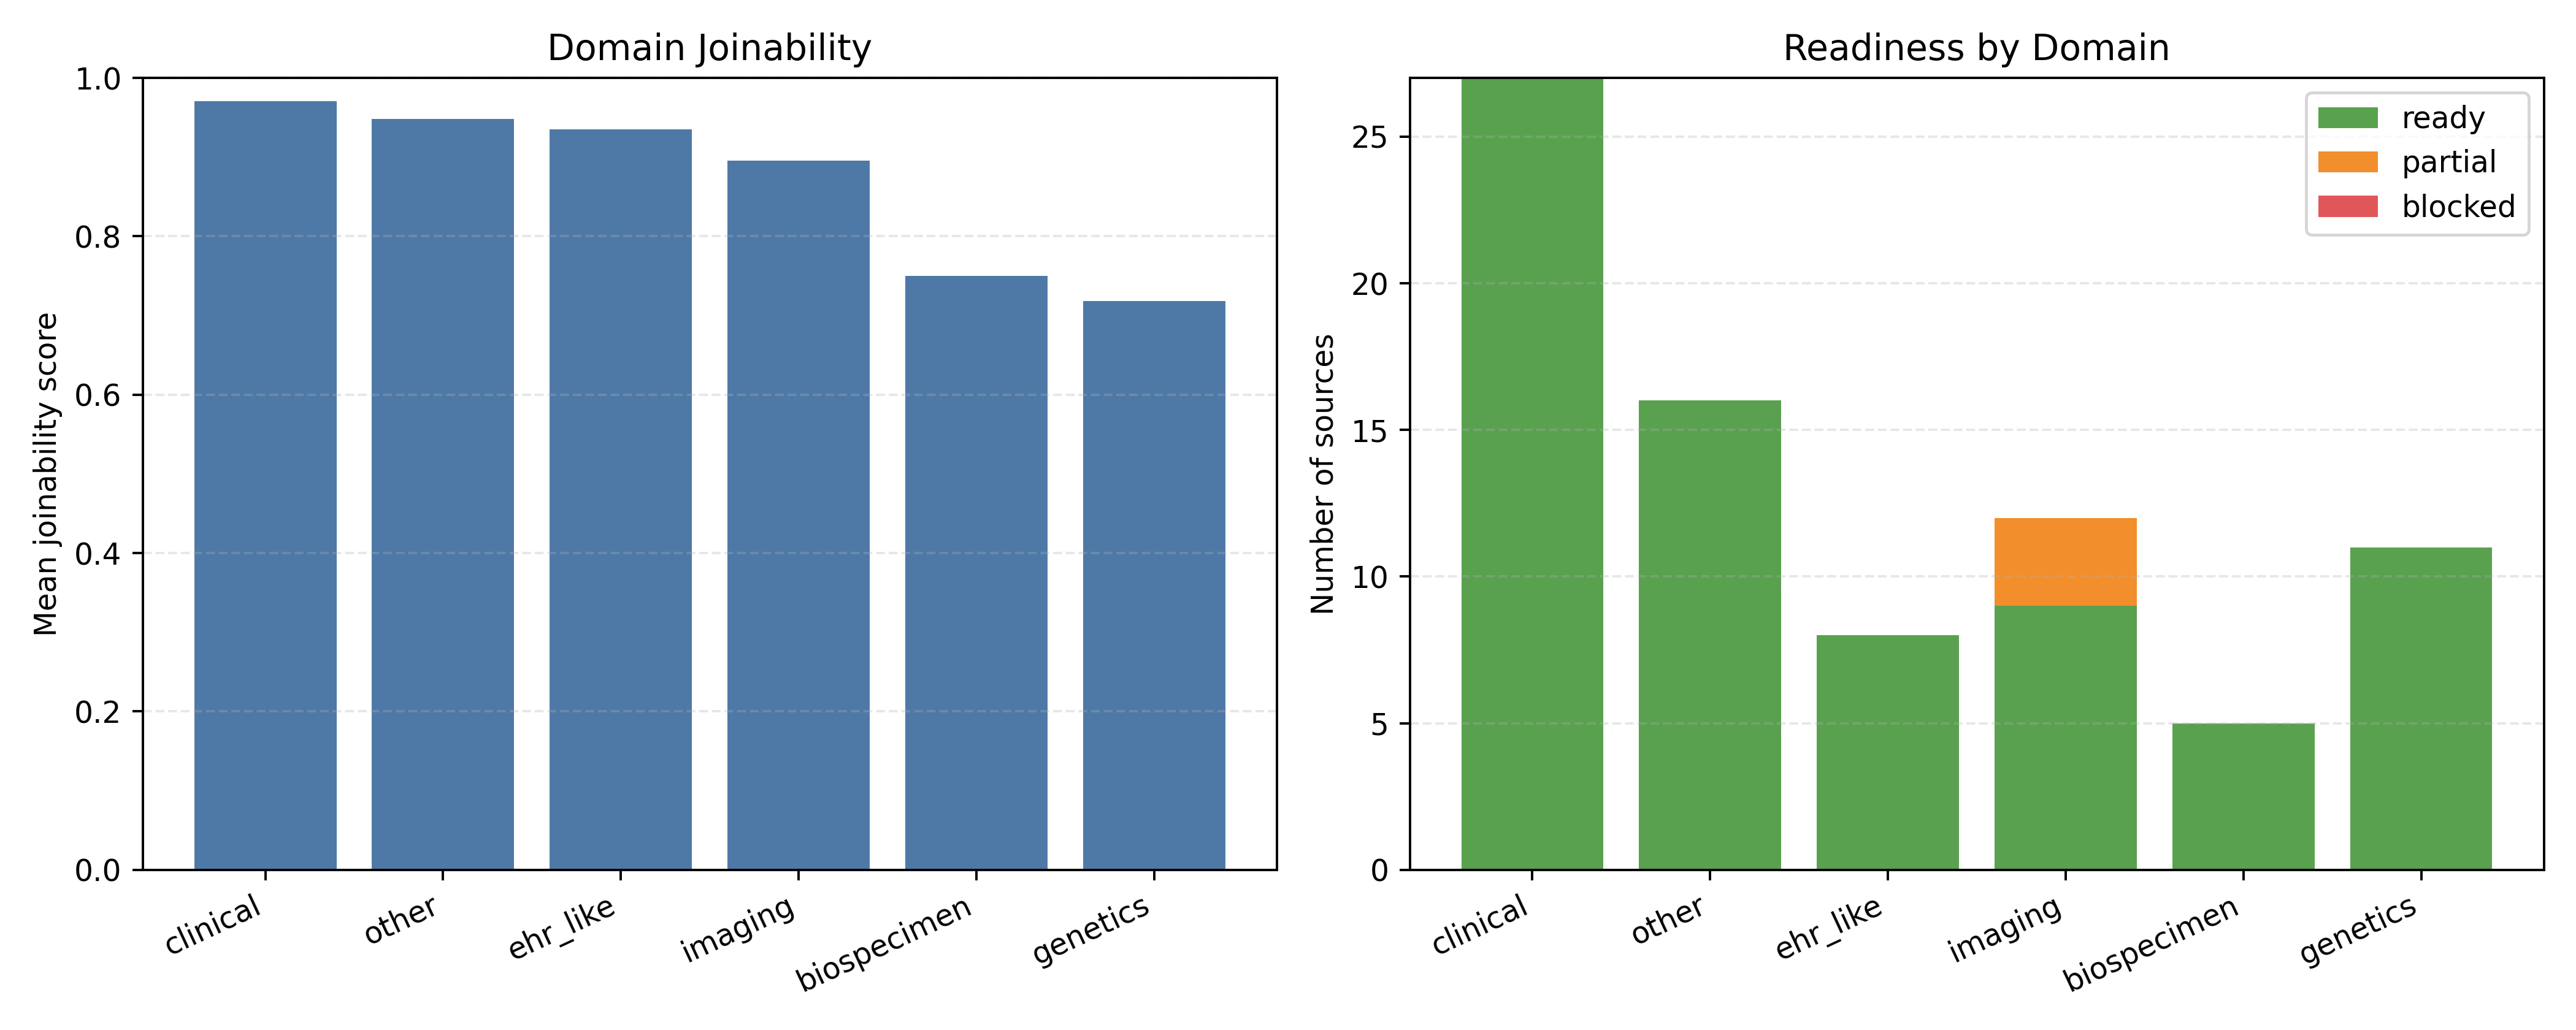
\includegraphics[width=0.95\textwidth]{../../../visualizations/publication_ieee/Figure05_Multimodal_Readiness.png}
\caption{Multimodal source-data readiness and joinability across PPMI domains.}
\label{fig:readiness}
\end{figure*}

\subsection{Cohort and endpoint contracts}
The final longitudinal analysis table used in the transparency audit contains 1,046 rows with 56 columns, median time-to-event of 18 months, and phenoconversion prevalence of 4.11\%. This severe imbalance motivates both explicit objective choices and calibration-focused reporting. Internal model development uses deterministic patient-level partitions to avoid leakage via repeated visits.

Across all runs reported here, the following contract is mandatory:
\begin{itemize}
\item patient key: \texttt{PATNO}
\item survival targets: \texttt{time}, \texttt{event}
\item classification target: \texttt{saa\_label}
\item fixed feature ordering and hash-locked schema metadata.
\end{itemize}
This contract prevents event-label substitution as a proxy classification target and stabilizes reproducibility across reruns and pull-based evaluations.

\subsection{External pull protocol}
External-like evaluation is executed through a frozen-checkpoint protocol. New pulls are ingested under a file-map contract, normalized to the canonical schema, and scored without retraining. This design enforces transportability testing rather than re-optimization, which is critical for honest clinical-readiness assessment.

\section{Methods}
\subsection{Problem formulation}
We model two tasks on a shared patient representation space: (i) binary SAA risk classification and (ii) time-to-event survival prediction when event variation is sufficient. Let each patient be represented by \(\mathbf{x}_i \in \mathbb{R}^{d}\), where \(d=50\) for the canonical run. A patient graph \(\mathcal{G}=(\mathcal{V},\mathcal{E})\) encodes population context through similarity edges.

\subsection{Graph and neuro-fuzzy model}
A multi-head graph attention encoder computes latent states:
\begin{equation}
\mathbf{h}'_i = \big\|_{k=1}^{K}\sigma\left(\sum_{j\in\mathcal{N}_i}\alpha^{k}_{ij}\mathbf{W}^{k}\mathbf{h}_j\right),
\end{equation}
where \(\alpha^{k}_{ij}\) are learned attention weights \cite{velickovic2018graph}. The neuro-fuzzy head then maps graph embeddings to rule-level activations via smooth membership functions. Defuzzified logits are computed as weighted combinations of consequent functions, enabling end-to-end optimization while retaining interpretable rule structure \cite{jang1993anfis,zadeh1965fuzzy}.

Compared with crisp graph heads, this design is intended to reduce unstable decision-boundary behavior under measurement noise and to provide clinician-readable intermediate reasoning signals.

\subsection{Training and baseline protocol}
FUZZY GIMAN is benchmarked against logistic regression, random forest, and SVM-RBF under the same deterministic split. Classification reporting includes AUC, PR-AUC, expected calibration error (ECE), Brier score, and confidence intervals. Survival reporting is separate and conditional on sufficient event variation.

Class imbalance is handled explicitly. In the current internal split, the training partition has 92 positives and 426 negatives (ratio 4.63:1). The pipeline supports focal-loss and class-weight mechanisms, and imbalance handling is tested as a first-class gate (C2), not as an afterthought.

\subsection{Explainability and governance cycles}
Explainability is evaluated using permutation importance and fuzzy rule-activation diagnostics. Governance is enforced through six automated cycles:
\begin{itemize}
\item C1 proxy dependency audit,
\item C2 imbalance and objective integrity,
\item C3 calibration review,
\item C4 digital twin sensitivity,
\item C5 metric contract separation,
\item C6 clinical readiness gate.
\end{itemize}
Each cycle emits machine-readable outputs and pass/fail logic.

\subsection{External-like validation and digital twin update cycle}
For \texttt{PPMI\_20251008\_REAL\_DISJOINT}, frozen checkpoint inference is run with no retraining. External metrics, calibration, subgroup diagnostics, and decision-curve outputs are generated with run-tagged provenance. A companion digital twin update-cycle script computes pull-to-baseline deltas, identifies changed patients, and records bounded intervention sensitivity summaries.

\section{Results}
\subsection{Internal discrimination and calibration}
Table~\ref{tab:internal_metrics} summarizes locked-split internal performance. FUZZY GIMAN has the strongest discrimination among compared models (AUC 0.590, PR-AUC 0.285), but raw probability calibration is poor (ECE 0.392, Brier 0.292). This distinction is critical: discrimination gains do not imply reliable probability estimates for clinical decision support.

Post-hoc calibration substantially improves internal reliability (Table~\ref{tab:calibration}). Isotonic regression achieves the lowest ECE (0.018), while Platt scaling achieves the best Brier score (0.145). These complementary results justify reporting both discrimination and calibration families together.

\begin{figure*}[!t]
\centering
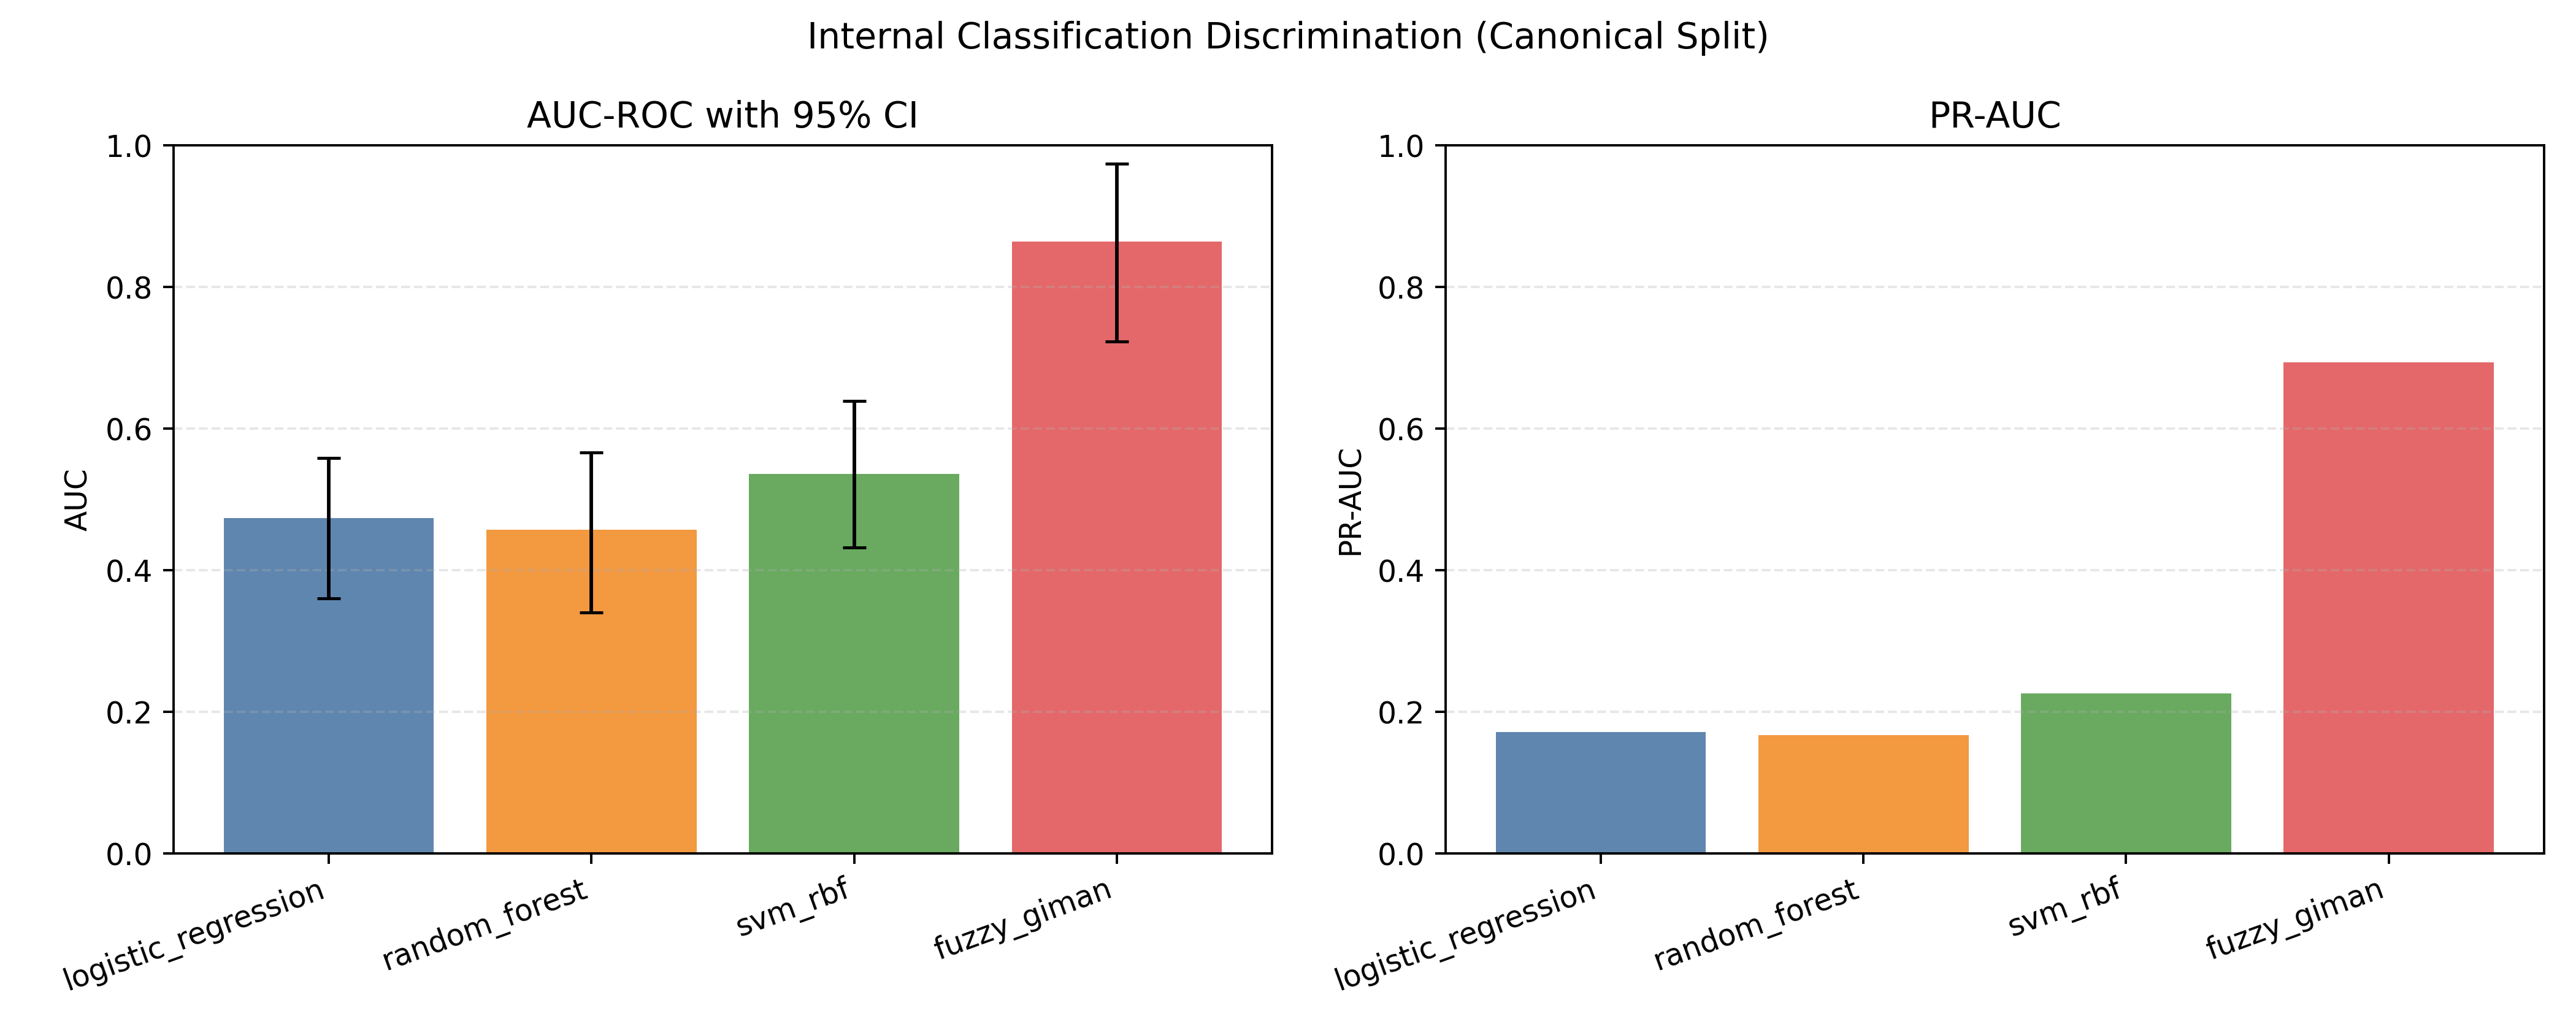
\includegraphics[width=0.95\textwidth]{../../../visualizations/publication_ieee/Figure01_Internal_Discrimination.png}
\caption{Internal discrimination metrics under canonical patient-level split.}
\label{fig:internal_discrimination}
\end{figure*}

\begin{table}[!t]
\centering
\caption{Internal classification metrics on canonical patient split.}
\label{tab:internal_metrics}
\begin{tabular}{lccccc}
\toprule
Model & AUC & AUC 95\% CI & PR-AUC & ECE & Brier \\
\midrule
logistic regression & 0.473 & [0.360, 0.559] & 0.172 & 0.338 & 0.267 \\
random forest & 0.457 & [0.340, 0.566] & 0.167 & 0.305 & 0.236 \\
svm\_rbf & 0.536 & [0.432, 0.639] & 0.226 & 0.003 & 0.145 \\
FUZZY GIMAN & 0.590 & [0.464, 0.719] & 0.285 & 0.392$^*$ & 0.292$^*$ \\
\bottomrule
\end{tabular}
\\
\footnotesize{$^*$Raw probabilities before post-hoc calibration.}
\end{table}

\begin{figure}[!t]
\centering
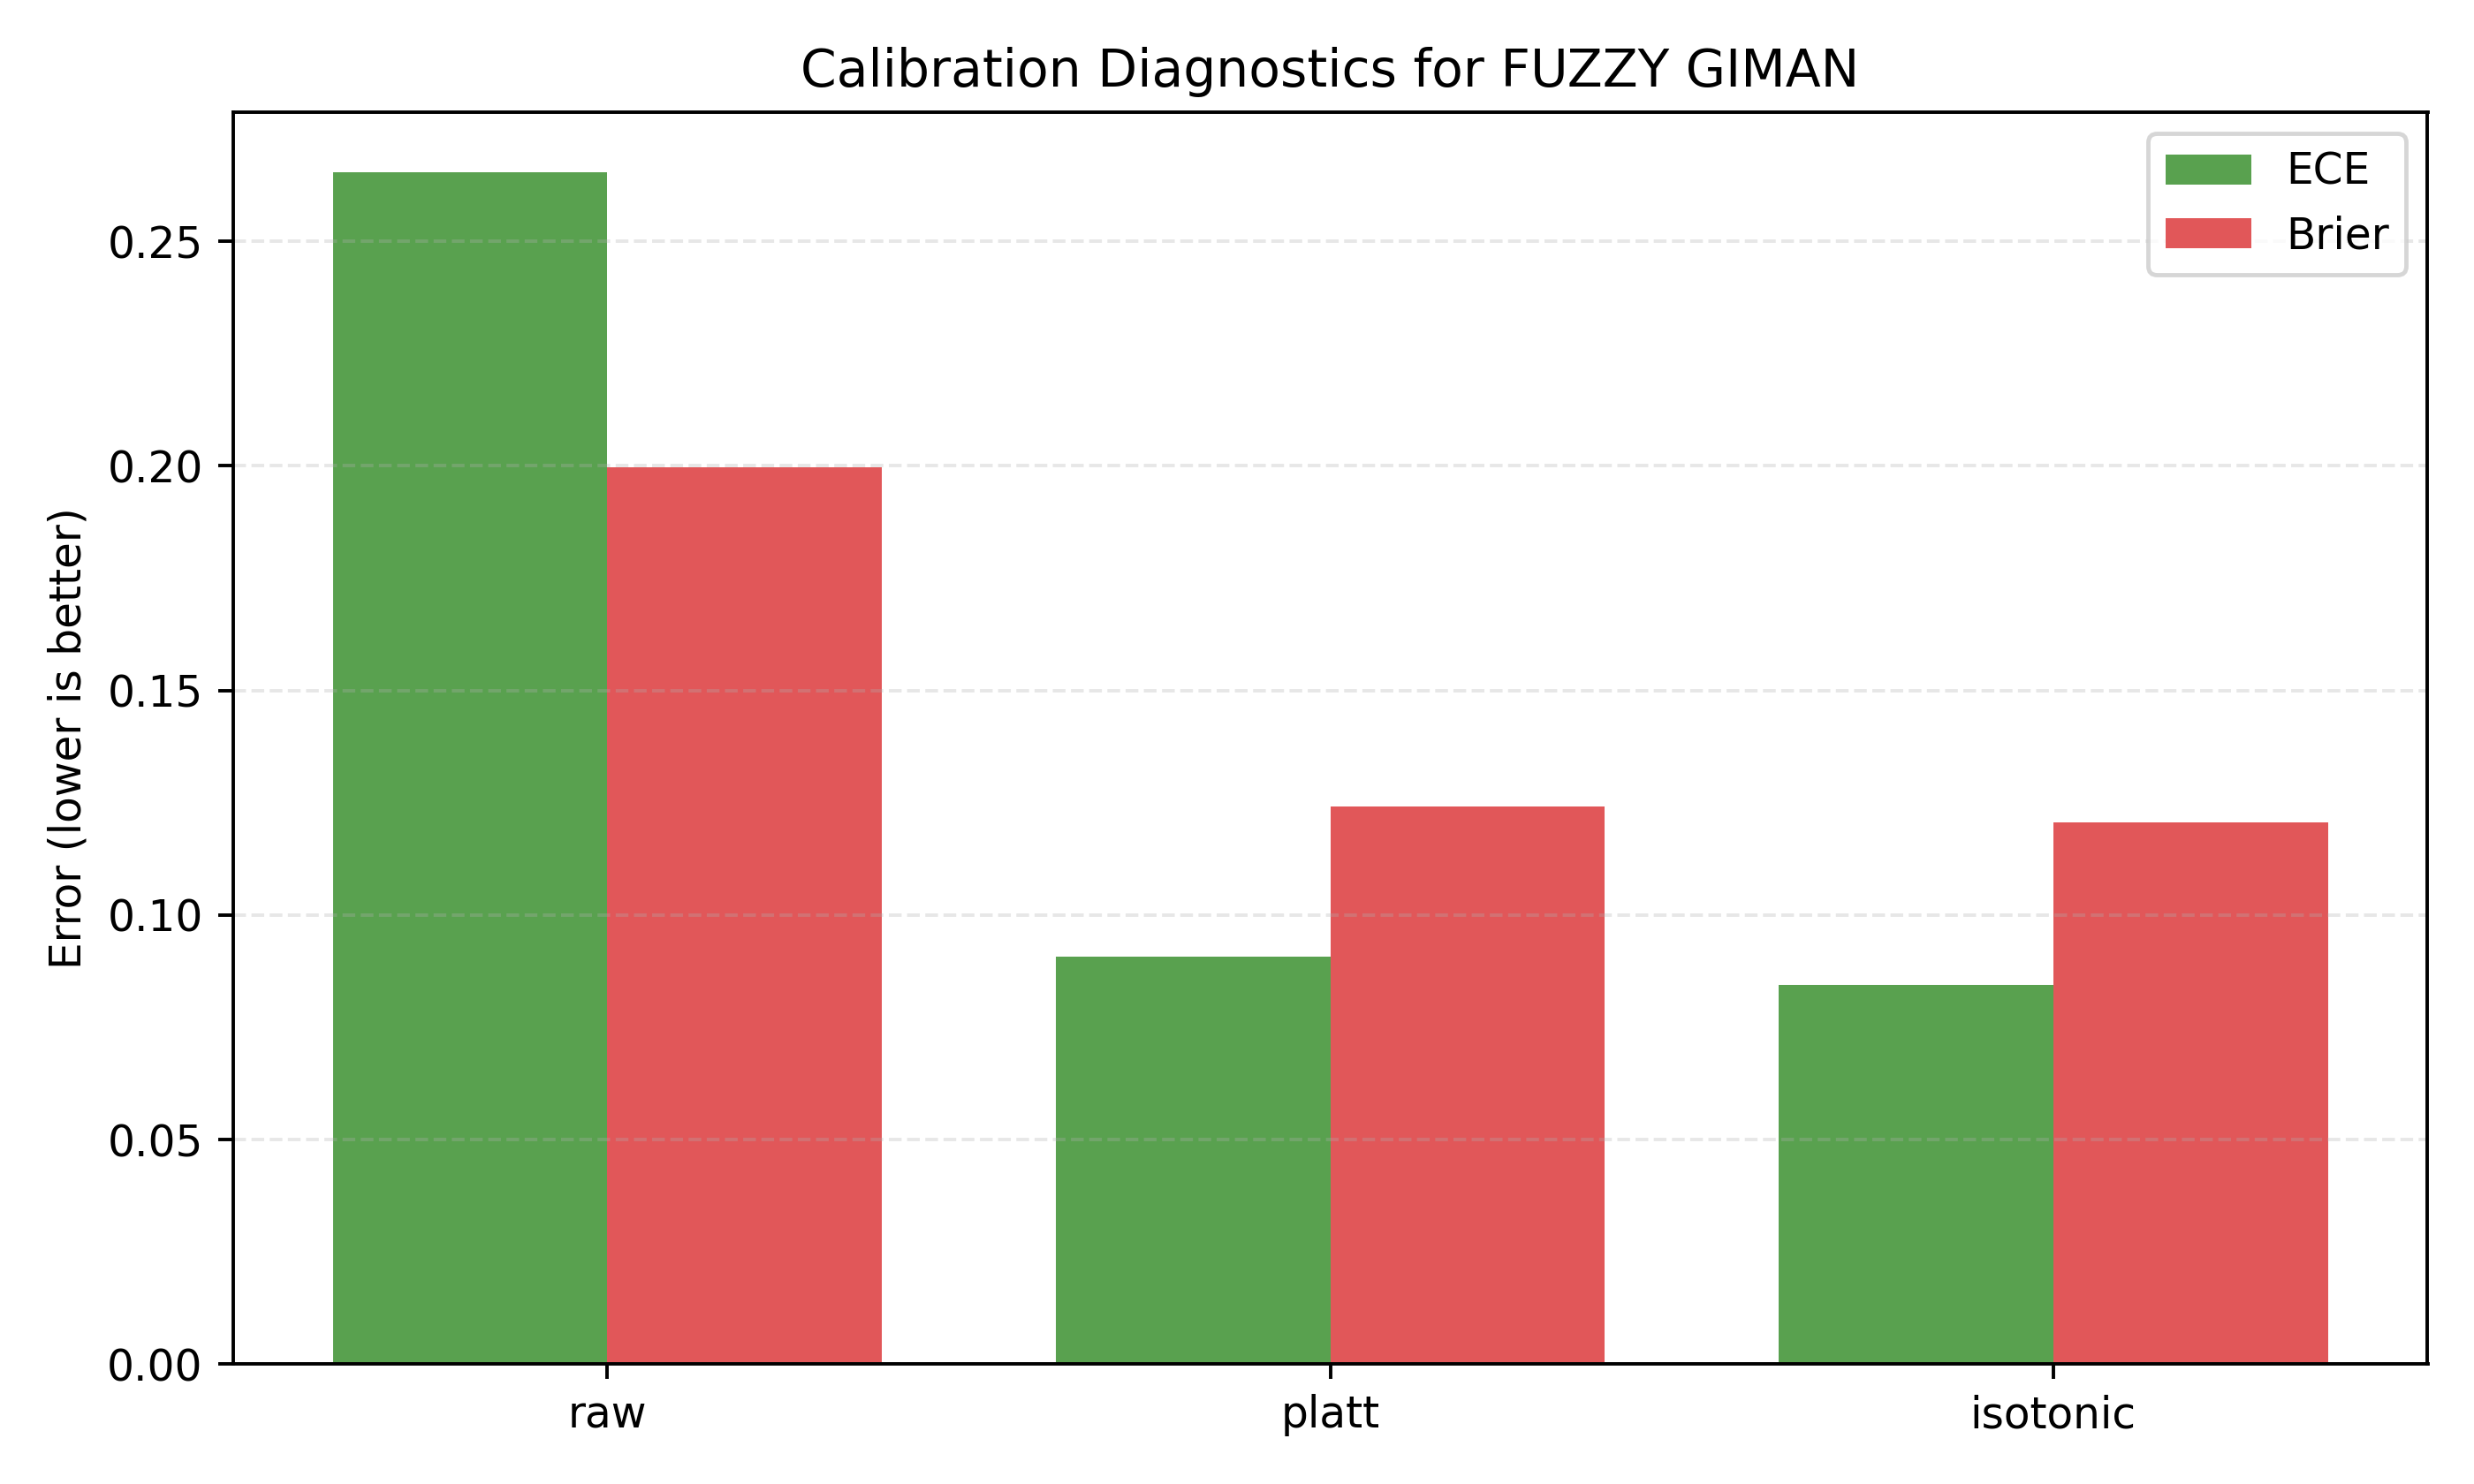
\includegraphics[width=\columnwidth]{../../../visualizations/publication_ieee/Figure02_Fuzzy_Calibration.png}
\caption{FUZZY GIMAN calibration diagnostics on held-out internal split.}
\label{fig:internal_calibration}
\end{figure}

\begin{table}[!t]
\centering
\caption{Post-hoc calibration effects for FUZZY GIMAN.}
\label{tab:calibration}
\begin{tabular}{lcc}
\toprule
Method & ECE (lower better) & Brier (lower better) \\
\midrule
Raw & 0.392 & 0.292 \\
Platt & 0.030 & 0.145 \\
Isotonic & 0.018 & 0.154 \\
\bottomrule
\end{tabular}
\end{table}

\subsection{Explainability and preprocessing transparency}
Explainability artifacts are generated from real-data outputs and include feature permutation importance and rule-activation diagnostics. In the latest audited internal run, the C1 proxy-dependency cycle passes with top feature \texttt{LRRK2} and a top-over-top10 dominance ratio of 0.127, indicating no single-feature collapse.

Preprocessing transparency confirms an imbalanced phenoconversion distribution (43 positives in 1,046 rows) and a discrete time-to-event structure concentrated at scheduled follow-up intervals. These characteristics contextualize performance variability and motivate both stratified evaluation and calibration review.

\begin{figure}[!t]
\centering
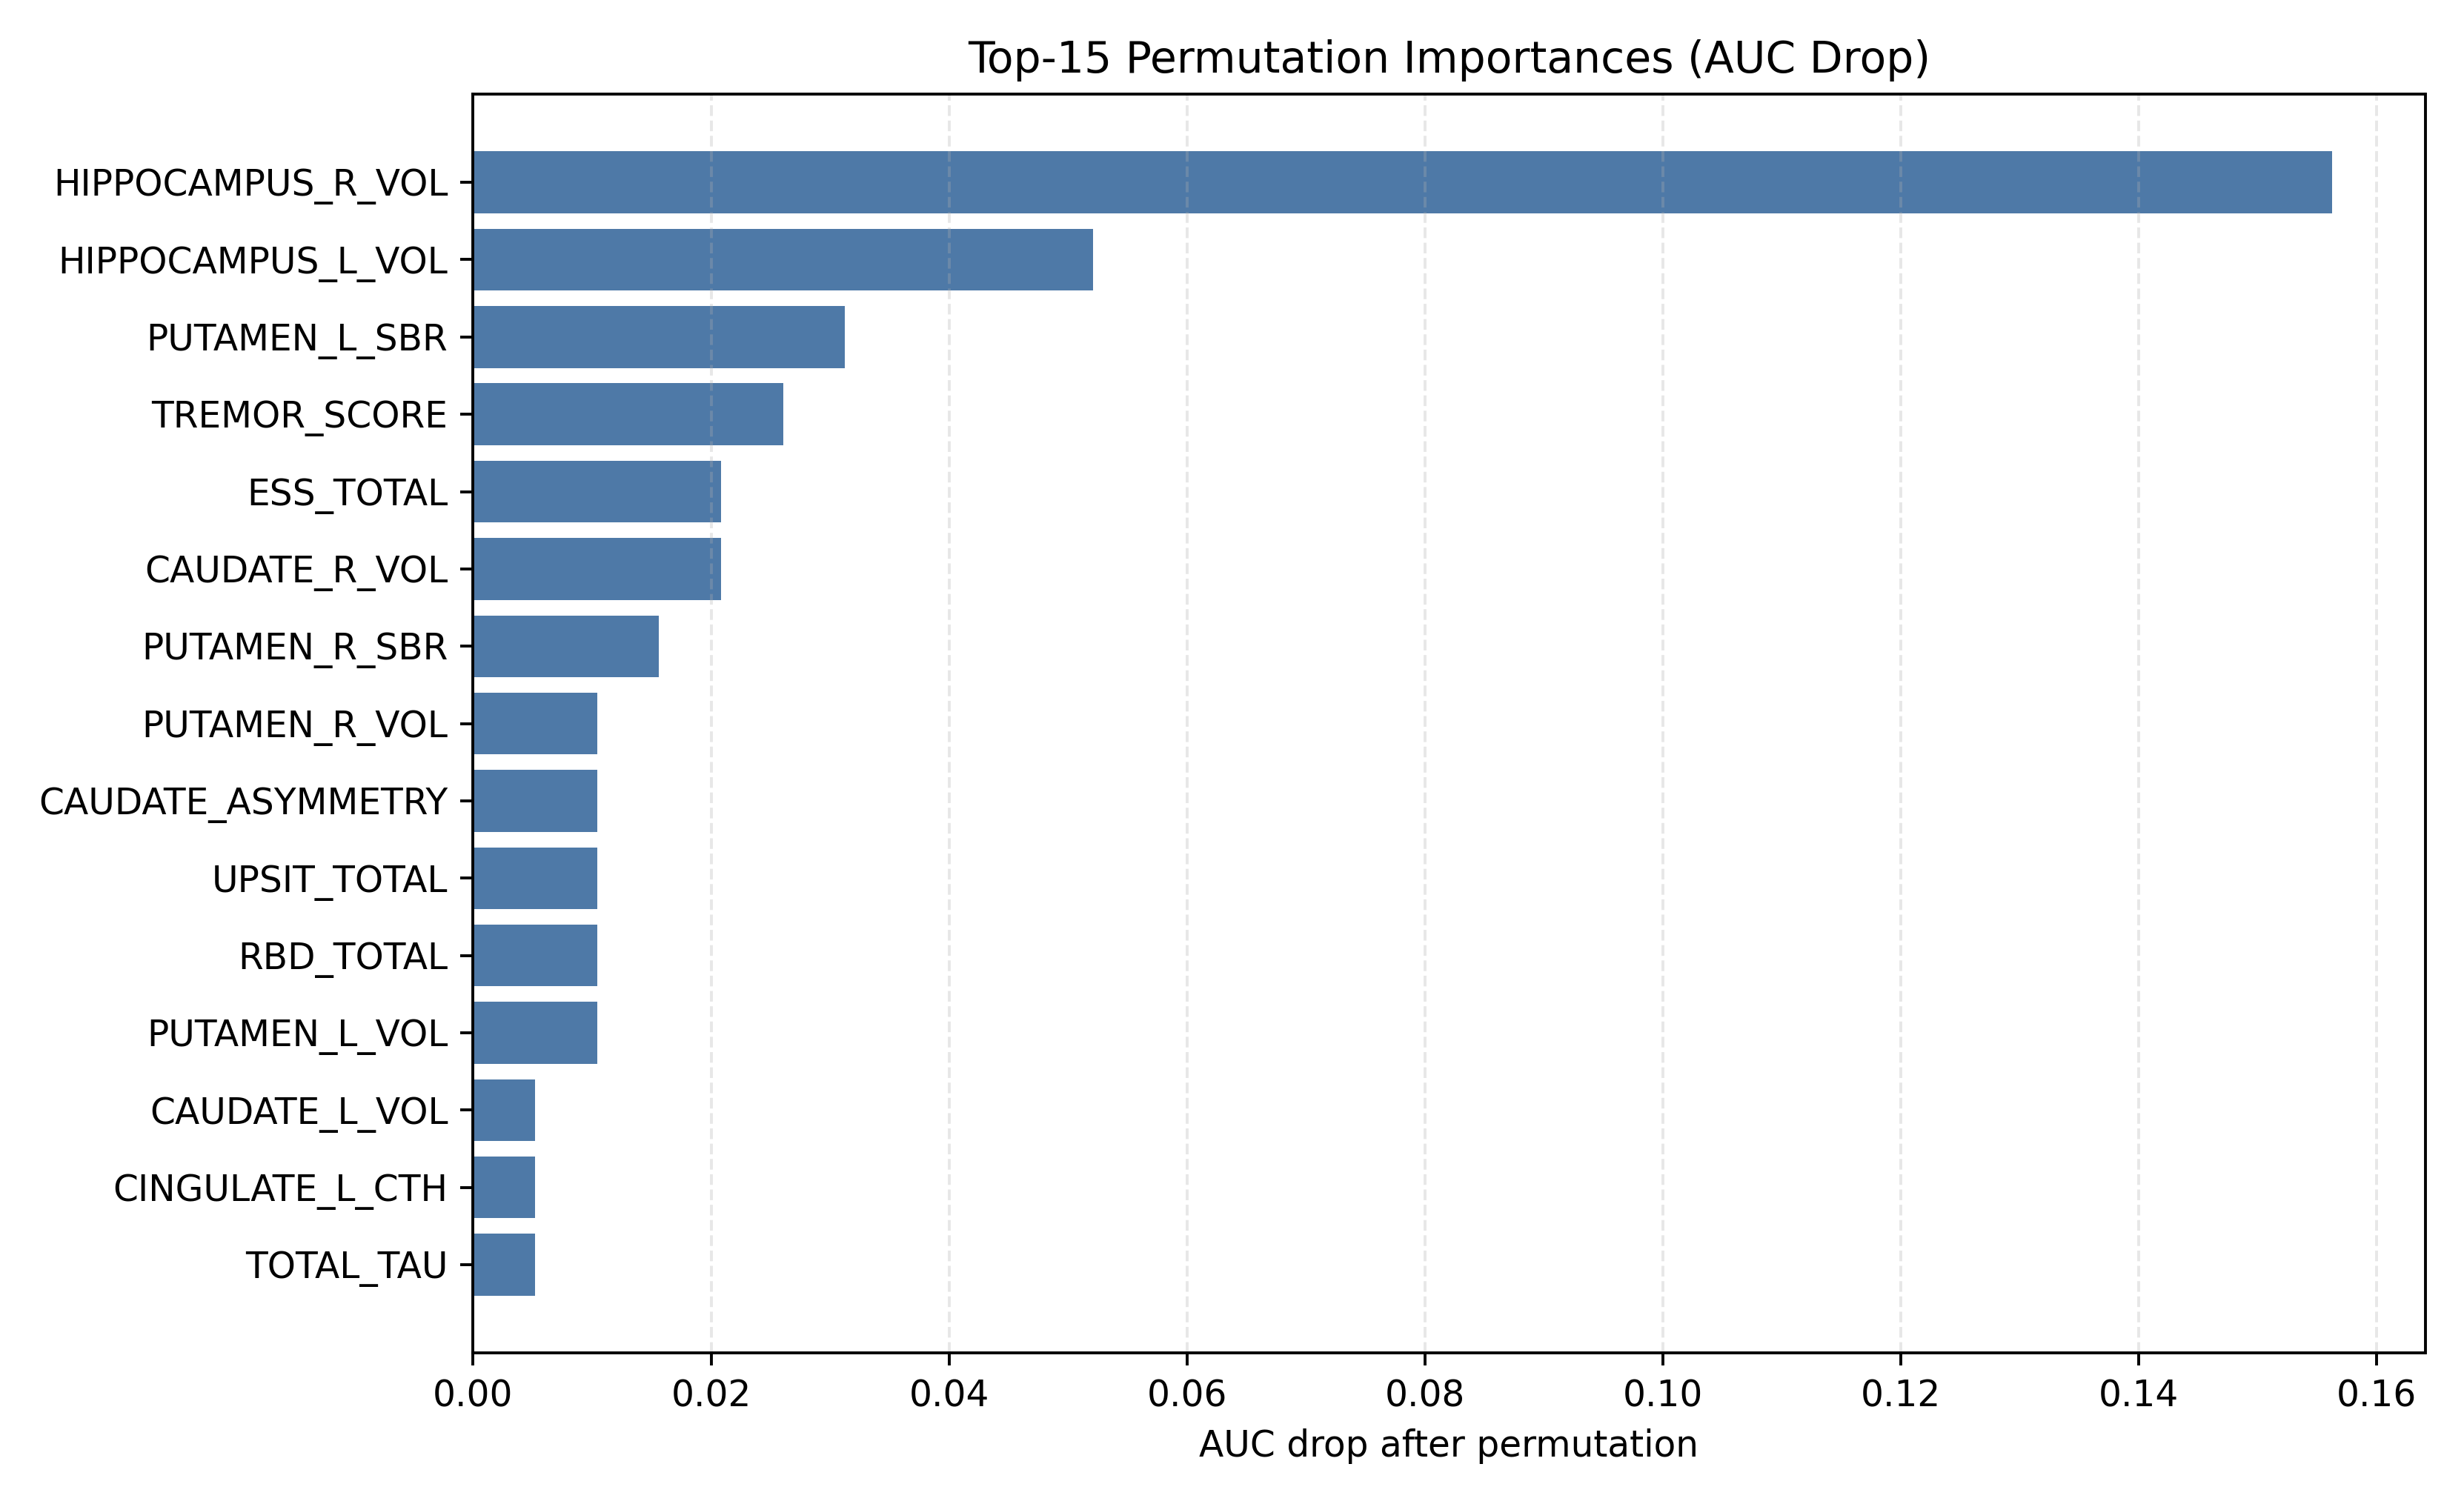
\includegraphics[width=\columnwidth]{../../../visualizations/publication_ieee/Figure03_Feature_Importance.png}
\caption{Feature-importance and fuzzy-rule explainability summary.}
\label{fig:importance}
\end{figure}

\begin{figure*}[!t]
\centering
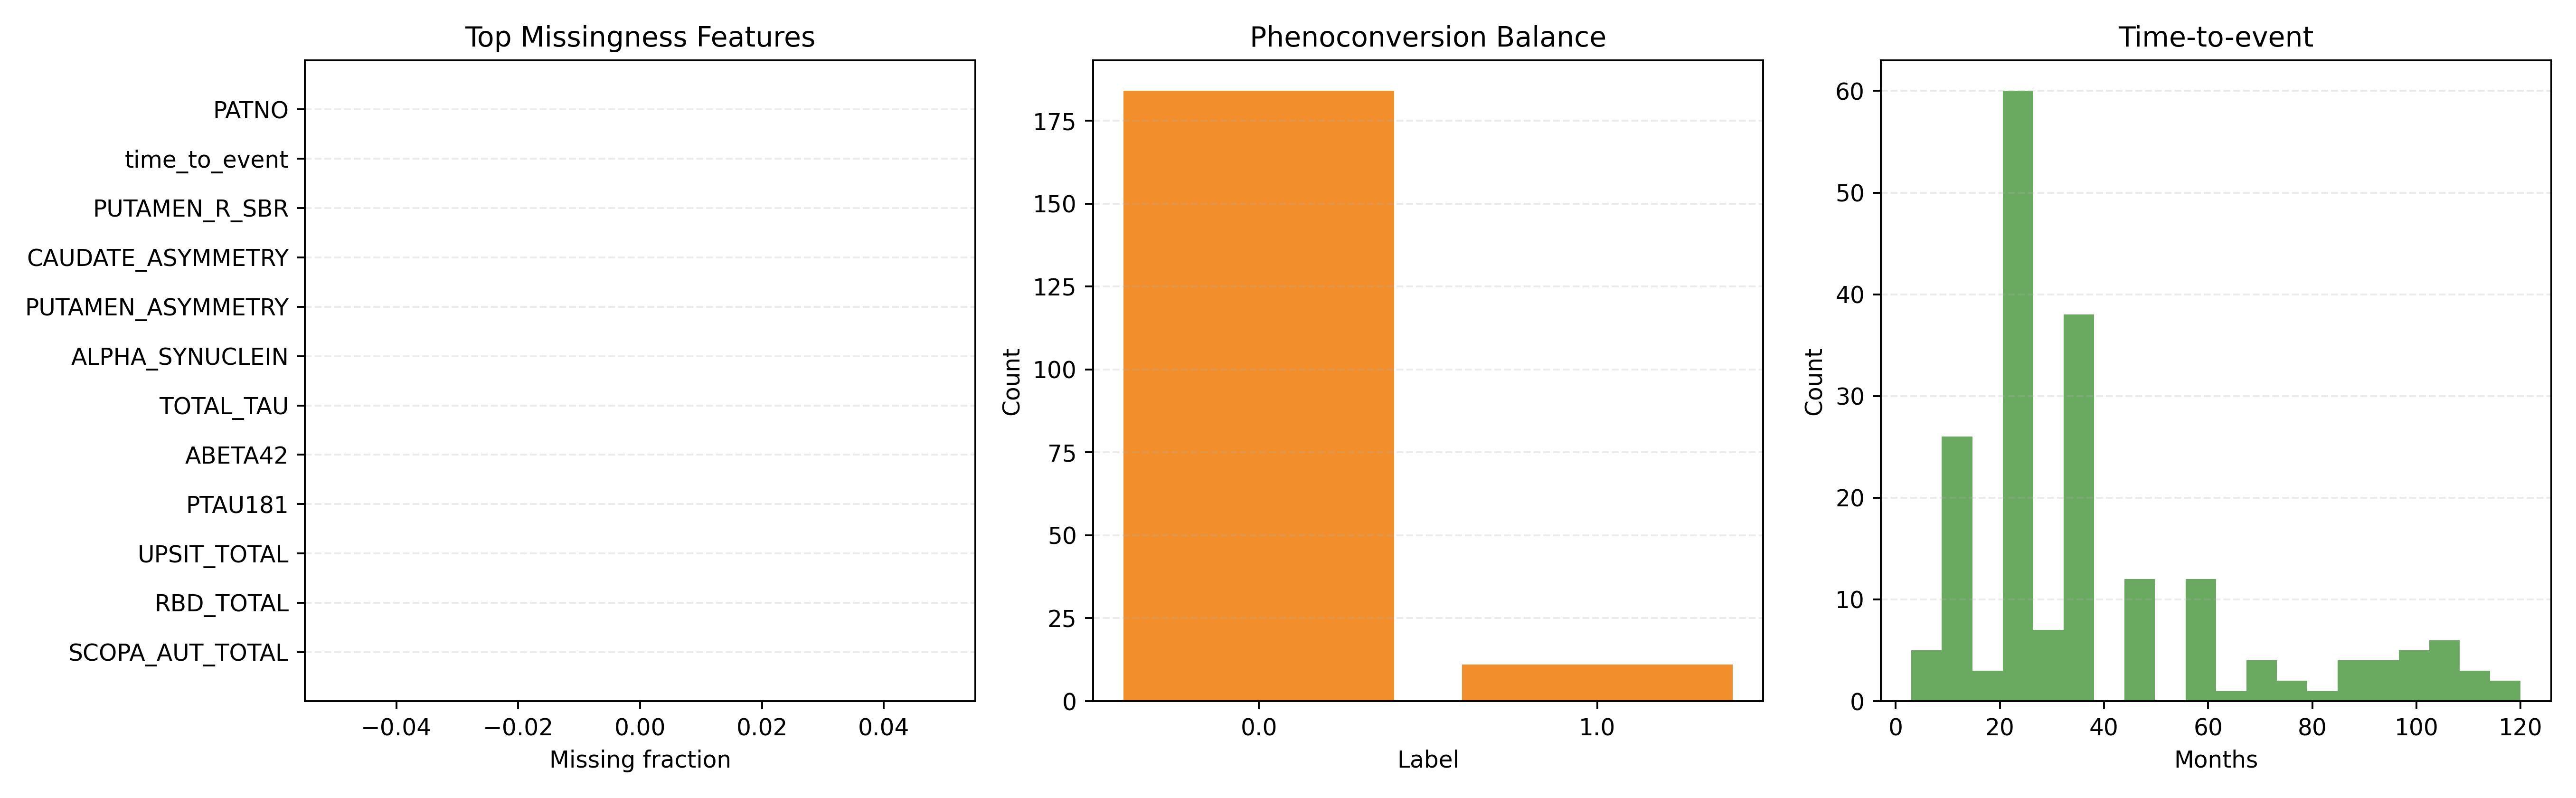
\includegraphics[width=0.95\textwidth]{../../../visualizations/publication_ieee/Figure06_Preprocessing_Transparency.png}
\caption{Preprocessing transparency panel for final longitudinal dataset.}
\label{fig:preprocess}
\end{figure*}

\subsection{Clinical hardening gate status}
All internal hardening cycles pass in the current audited run (Table~\ref{tab:gates}). This includes C3 calibration improvement checks and C4 digital twin sensitivity checks. For C4, moderate intervention scans show mean absolute delta risk of 0.00264 and stress scans 0.01429, indicating bounded but non-trivial response to perturbation scenarios.

The C6 gate now requires the presence of a run-tagged external validation artifact and real-data-only governance flags. This gate design prevents unsupported readiness language when external evidence is absent.

\begin{table}[!t]
\centering
\caption{Clinical hardening review cycles (latest audited run).}
\label{tab:gates}
\begin{tabular}{lc}
\toprule
Cycle & Status \\
\midrule
C1\_proxy\_dependency\_audit & PASS \\
C2\_imbalance\_and\_objective & PASS \\
C3\_calibration\_review & PASS \\
C4\_digital\_twin\_sensitivity & PASS \\
C5\_metric\_contract\_separation & PASS \\
C6\_clinical\_readiness\_gate & PASS \\
\bottomrule
\end{tabular}
\end{table}

\begin{figure}[!t]
\centering
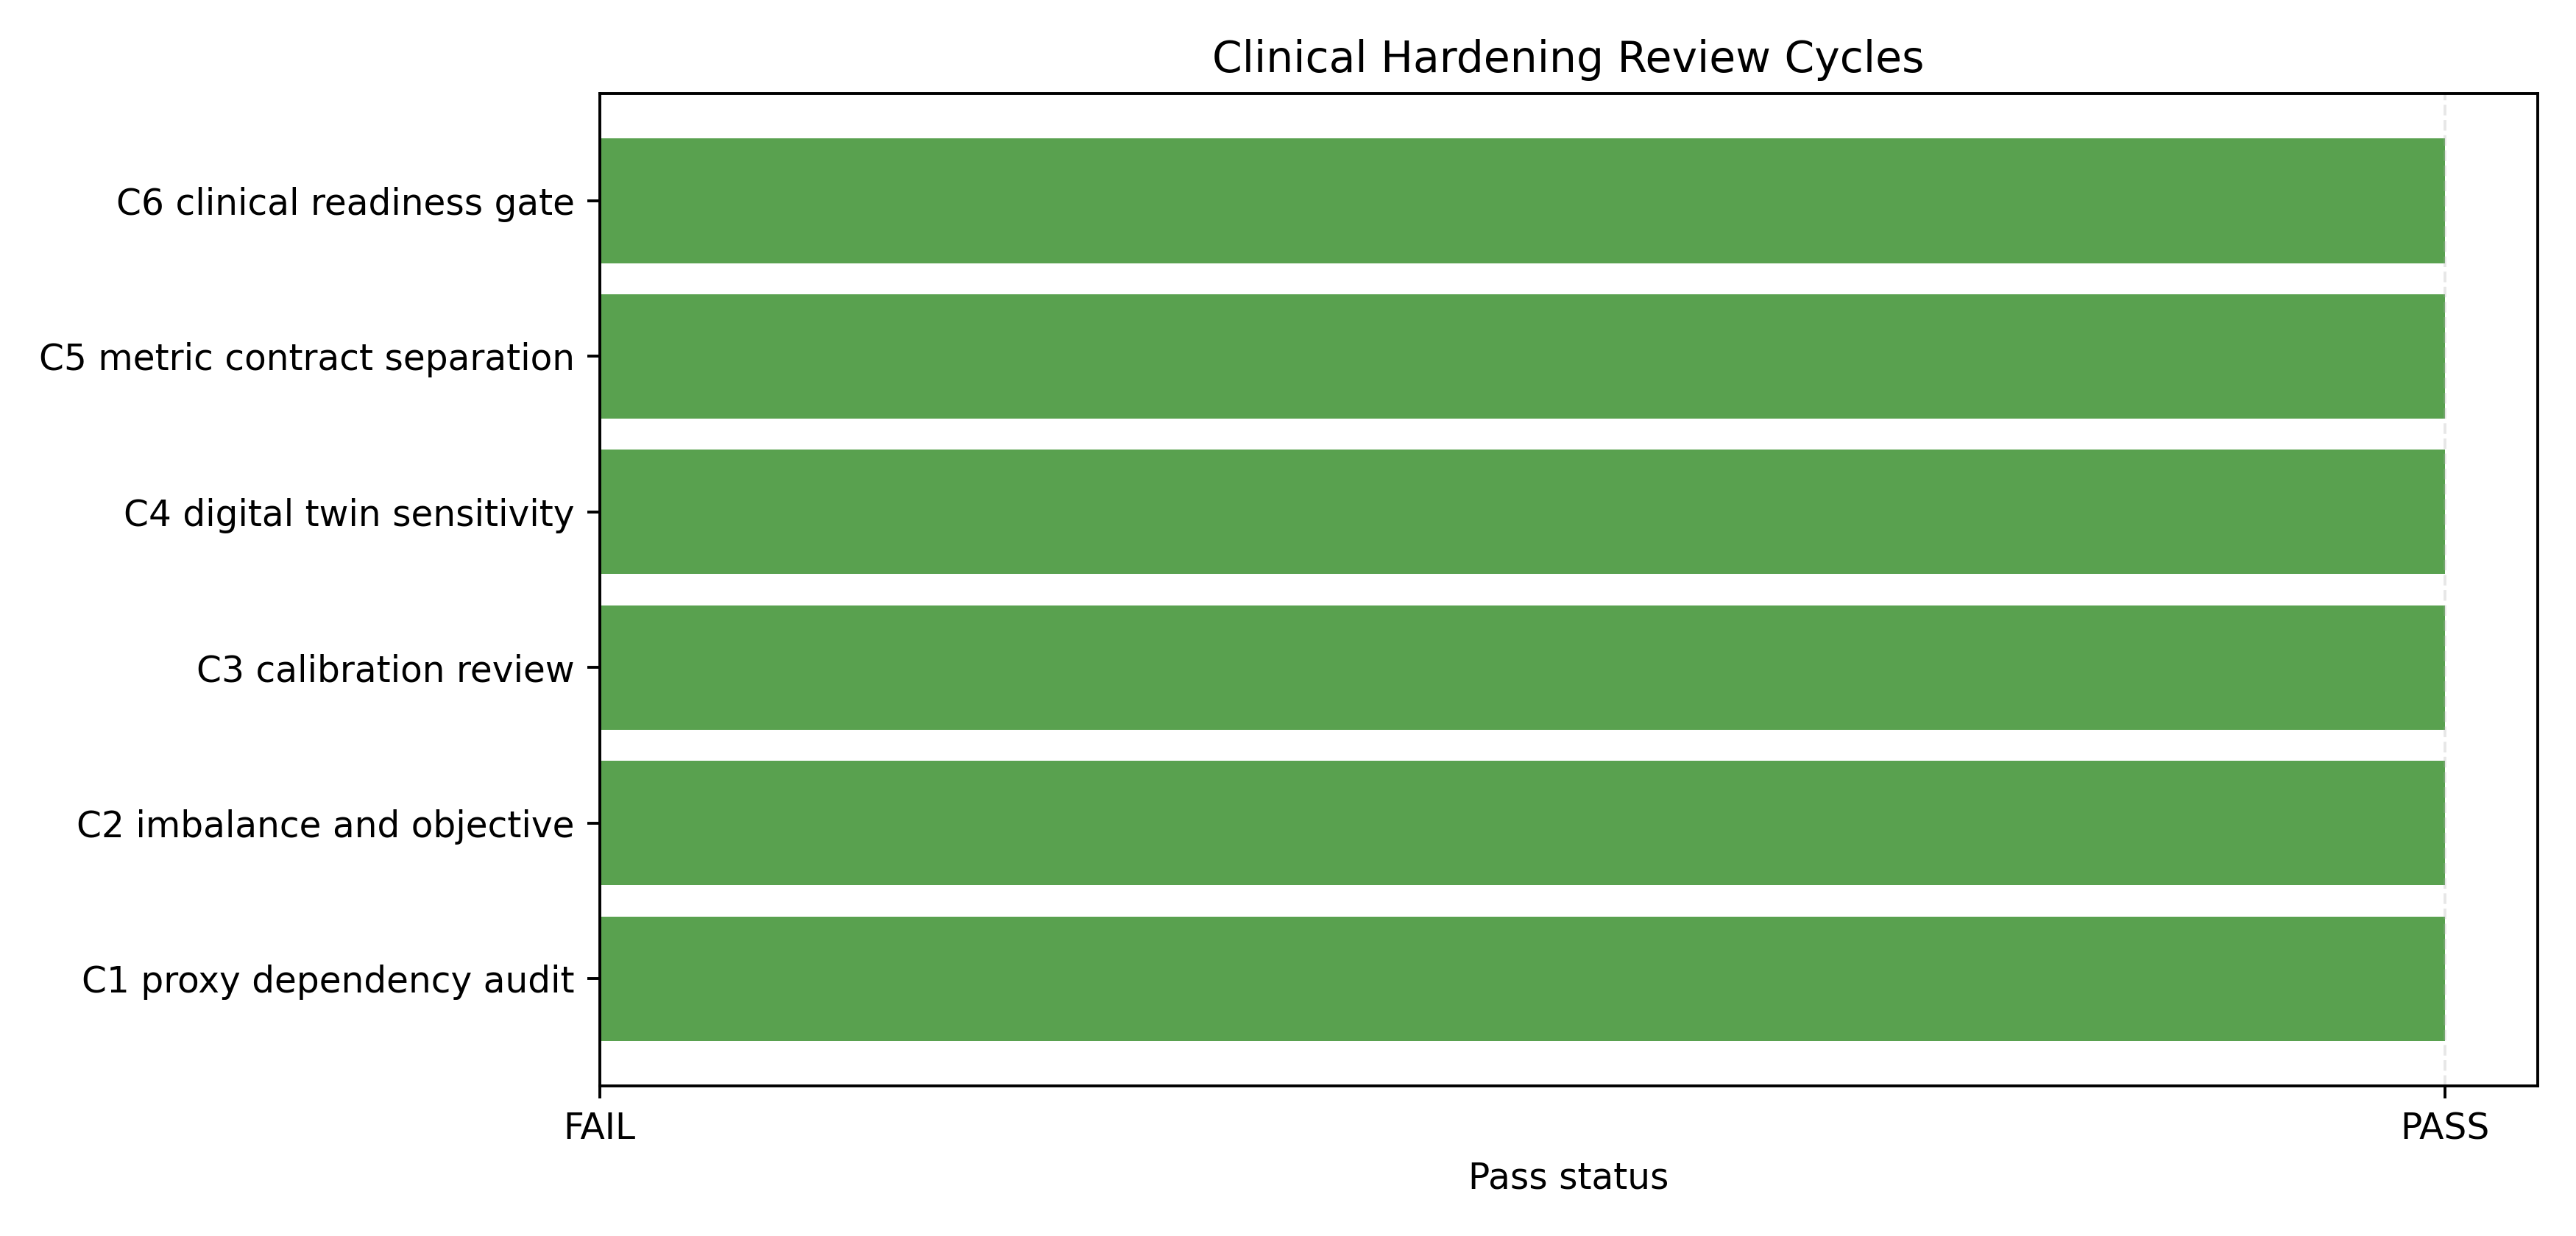
\includegraphics[width=\columnwidth]{../../../visualizations/publication_ieee/Figure07_Clinical_Gates.png}
\caption{Clinical hardening cycle outcomes (C1--C6).}
\label{fig:gates}
\end{figure}

\subsection{External-like validation and transportability}
Despite internal improvements, disjoint pull evaluation shows a substantial transportability drop. External-like metrics are AUC 0.316 (95\% CI 0.088--0.631) and PR-AUC 0.047 (95\% CI 0.021--0.117) on \(n=50\) with only three positive labels. Raw external calibration is weak (ECE 0.502, Brier 0.308); post-hoc methods improve both metrics but do not resolve discrimination limitations.

Survival discrimination is explicitly marked unavailable because external event variation is insufficient (\(n_{events}=0\)). Subgroup analysis is similarly constrained by missing demographic covariates and sparse genotype-positive counts. These are informative negative findings and should be interpreted as protocol outputs, not pipeline failures.

\begin{table}[!t]
\centering
\caption{External-like validation metrics (\texttt{PPMI\_20251008\_REAL\_DISJOINT}).}
\label{tab:external}
\begin{tabular}{lcc}
\toprule
Metric & Value & 95\% CI \\
\midrule
AUC & 0.316 & [0.088, 0.631] \\
PR-AUC & 0.047 & [0.021, 0.117] \\
C-index & N/A & N/A \\
\bottomrule
\end{tabular}
\end{table}

\begin{figure}[!t]
\centering
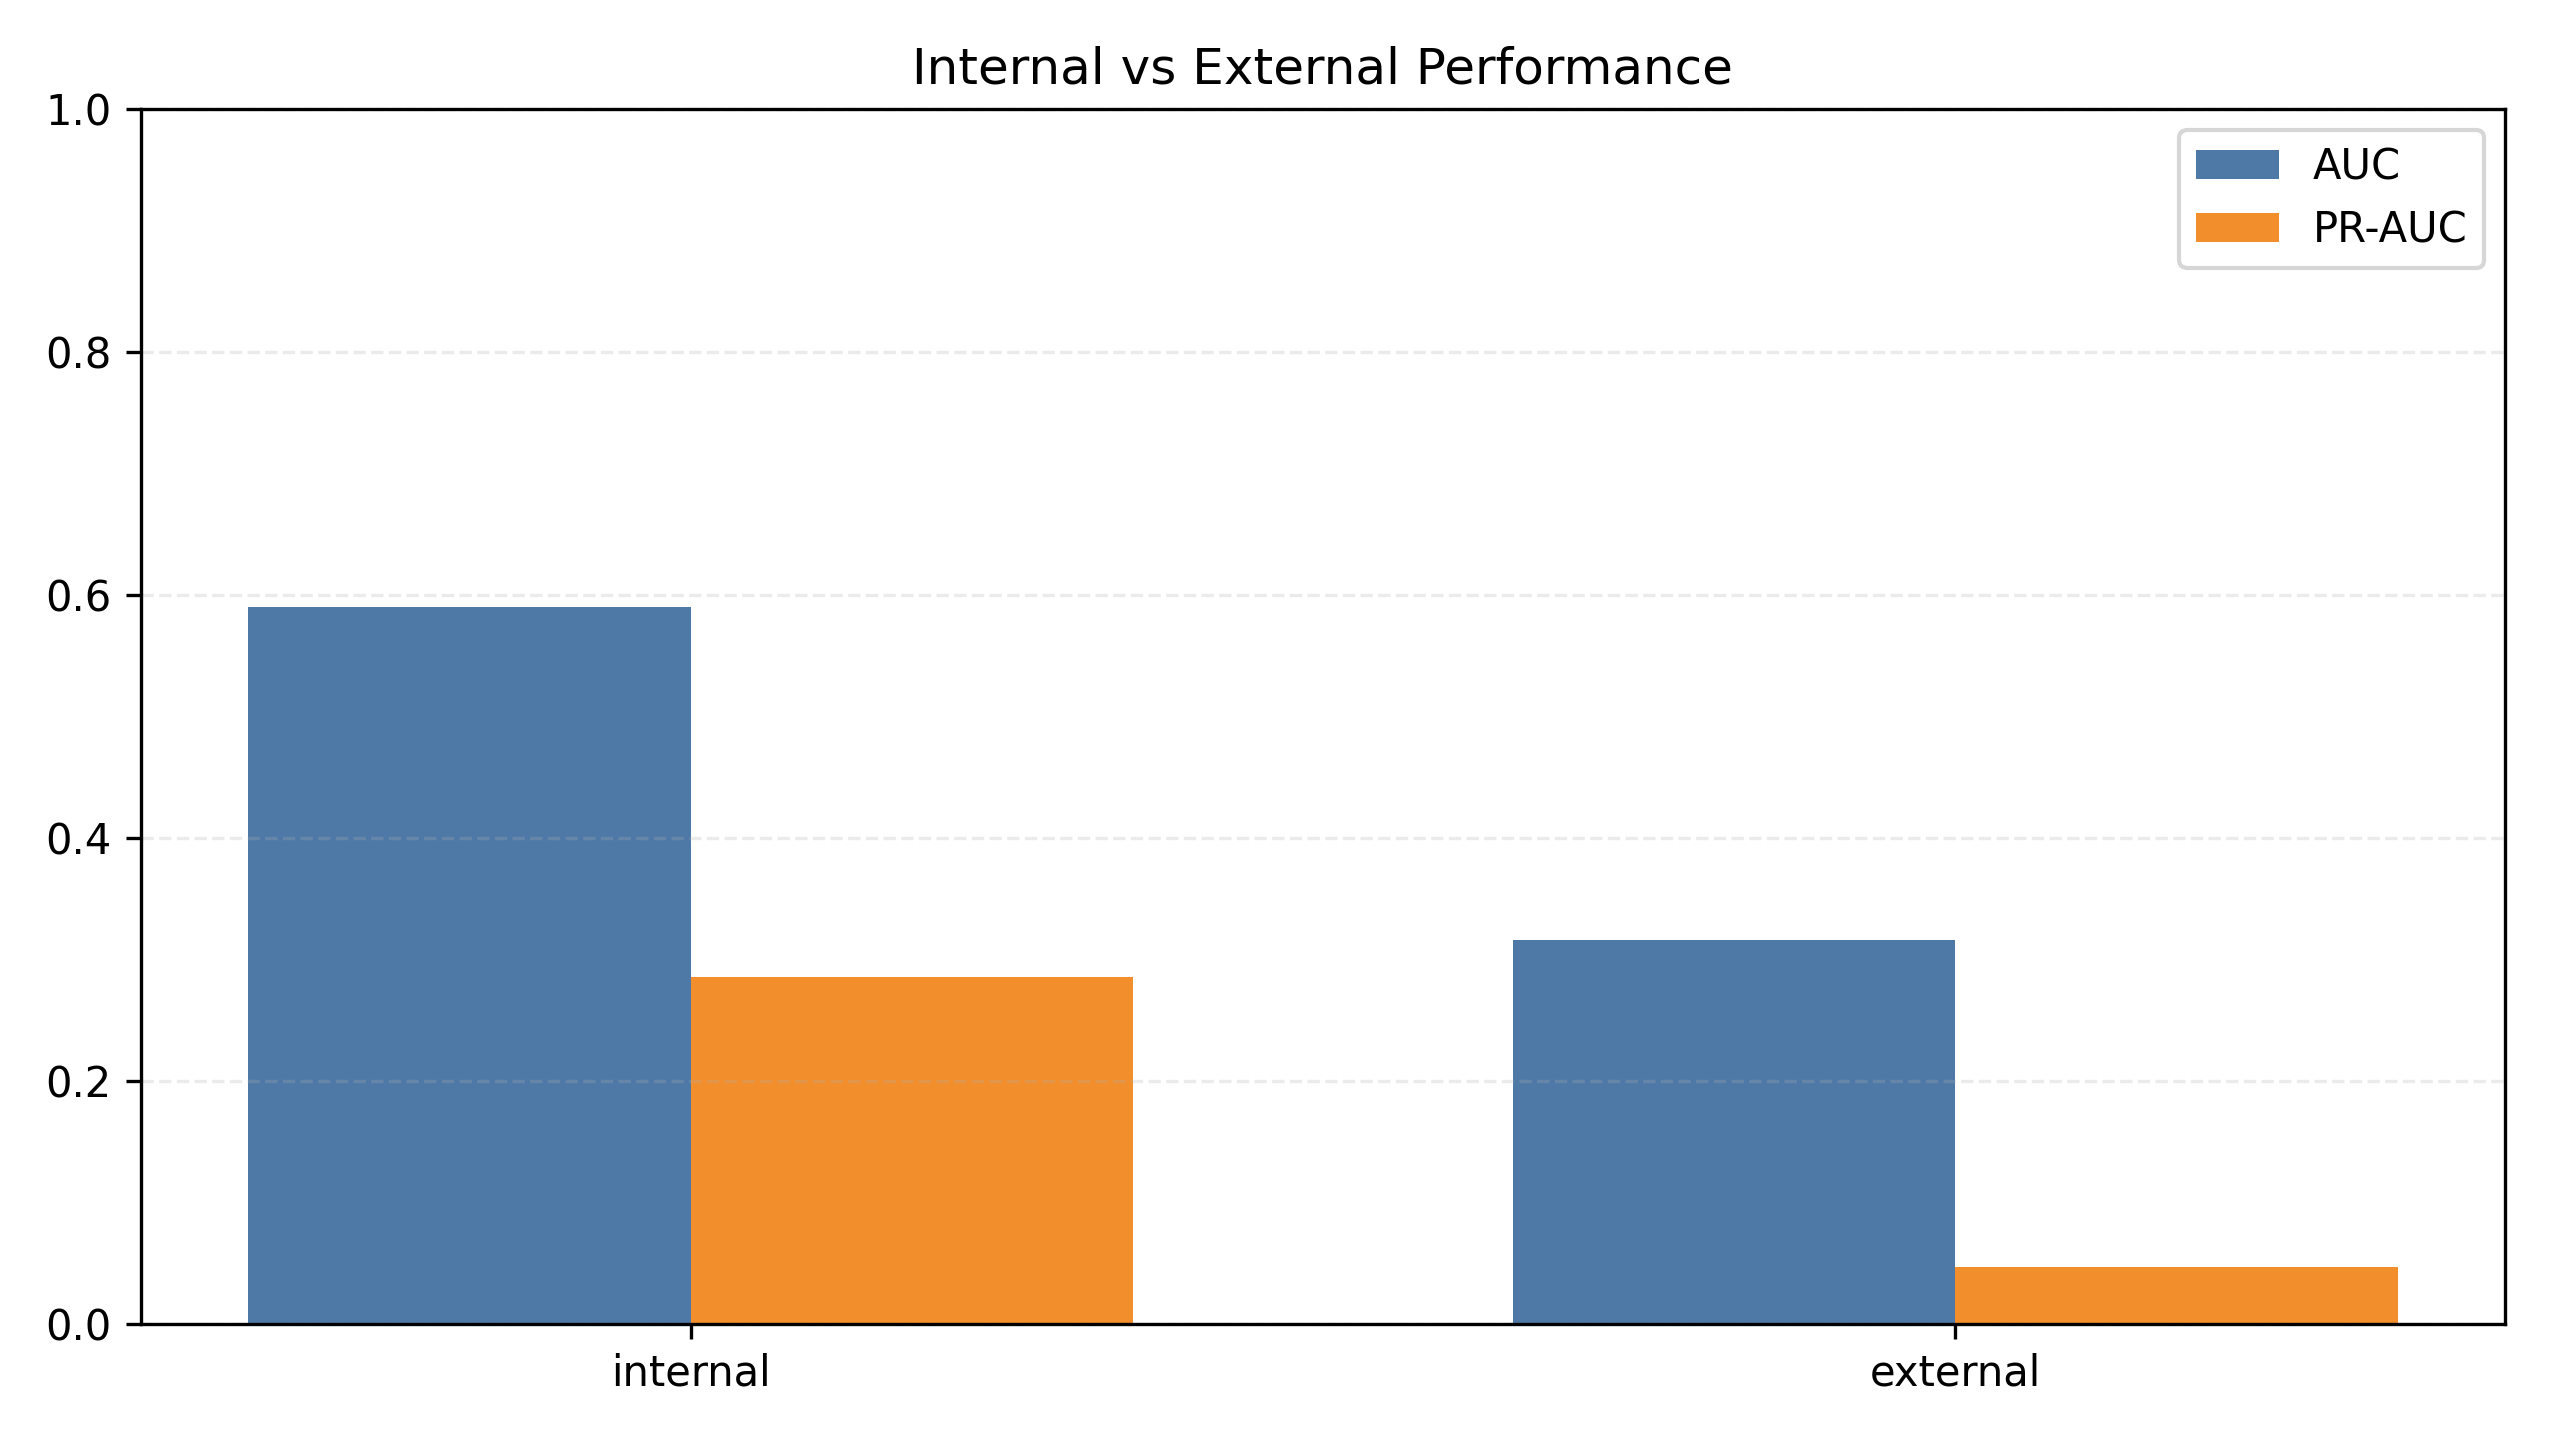
\includegraphics[width=\columnwidth]{../../../visualizations/publication_ieee_external/PPMI_20251008_REAL_DISJOINT/phase3_internal_vs_external_panel.png}
\caption{Internal vs. external-like comparison panel.}
\label{fig:int_ext}
\end{figure}

\begin{figure}[!t]
\centering
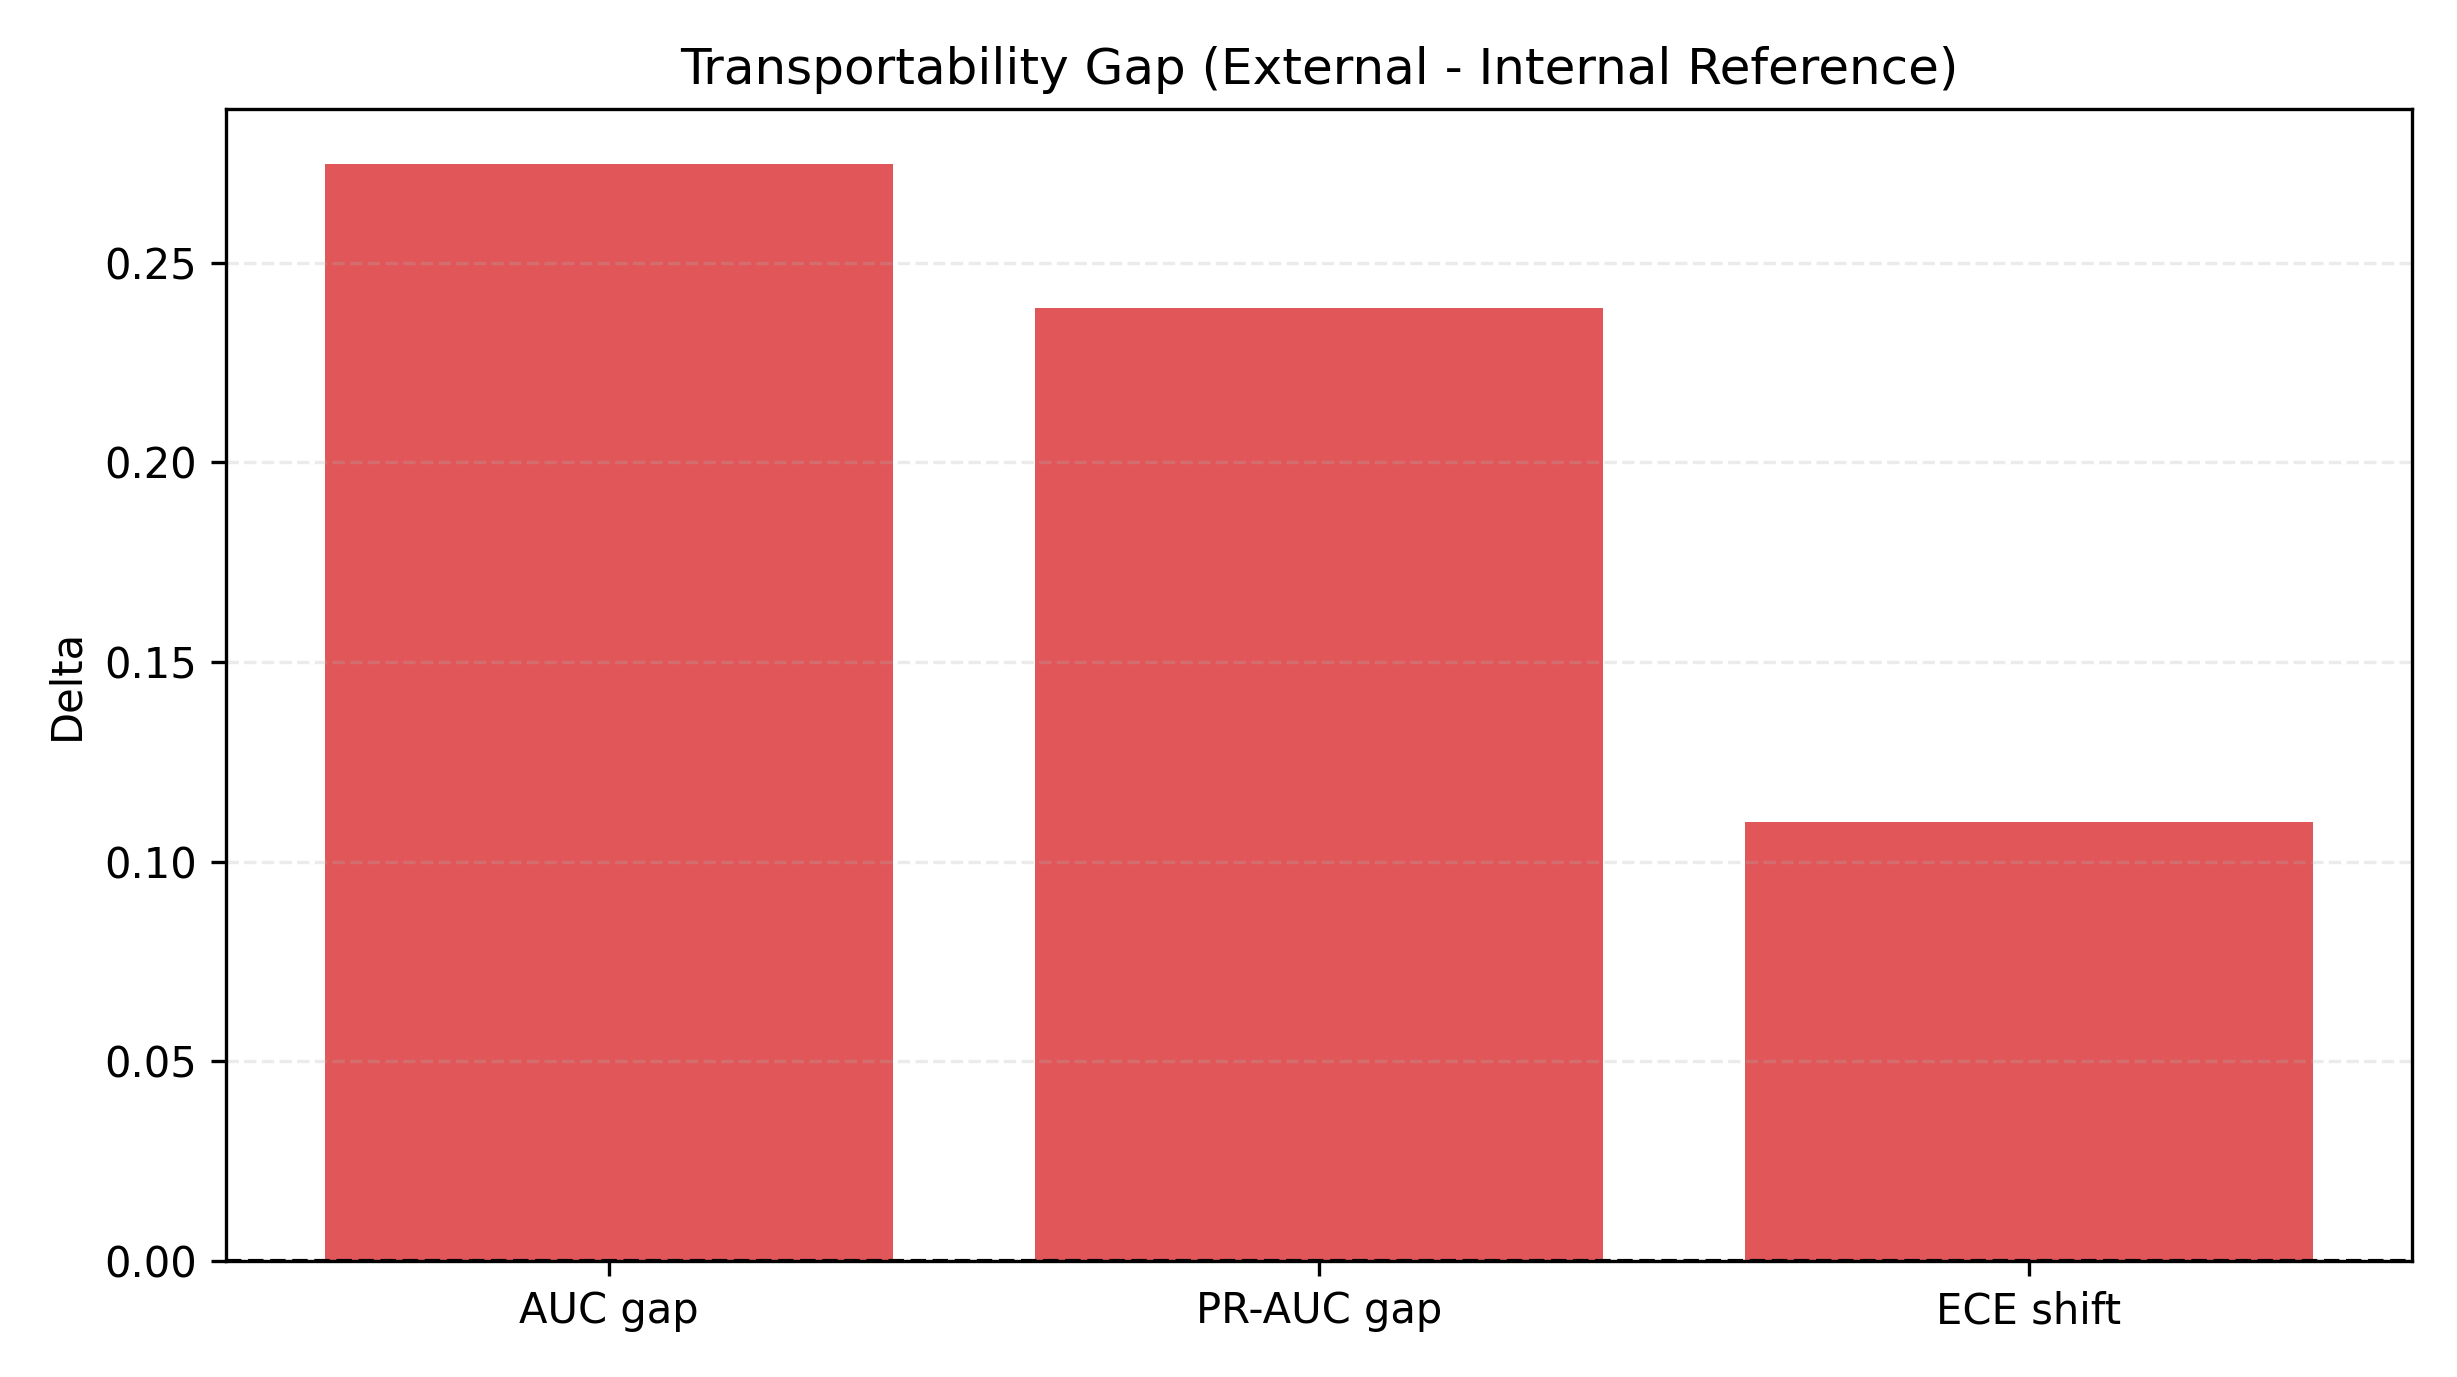
\includegraphics[width=\columnwidth]{../../../visualizations/publication_ieee_external/PPMI_20251008_REAL_DISJOINT/phase3_transportability_gap.png}
\caption{Transportability gap for external-like disjoint pull.}
\label{fig:transport}
\end{figure}

\subsection{Digital twin sensitivity and update readiness}
Digital twin sensitivity outputs remain bounded and deterministic under repeated execution. In the disjoint pull update cycle, no patient overlap with the baseline twin registry was observed (\texttt{n\_changed\_patients=0}); therefore, refresh deltas are correctly zero by construction. This behavior validates the update engine's guardrails for identity-disjoint ingestion scenarios.

Sensitivity summaries still provide meaningful signals for intervention-response profiling and establish a reusable contract for future pulls that do include overlapping patients.

\begin{figure*}[!t]
\centering
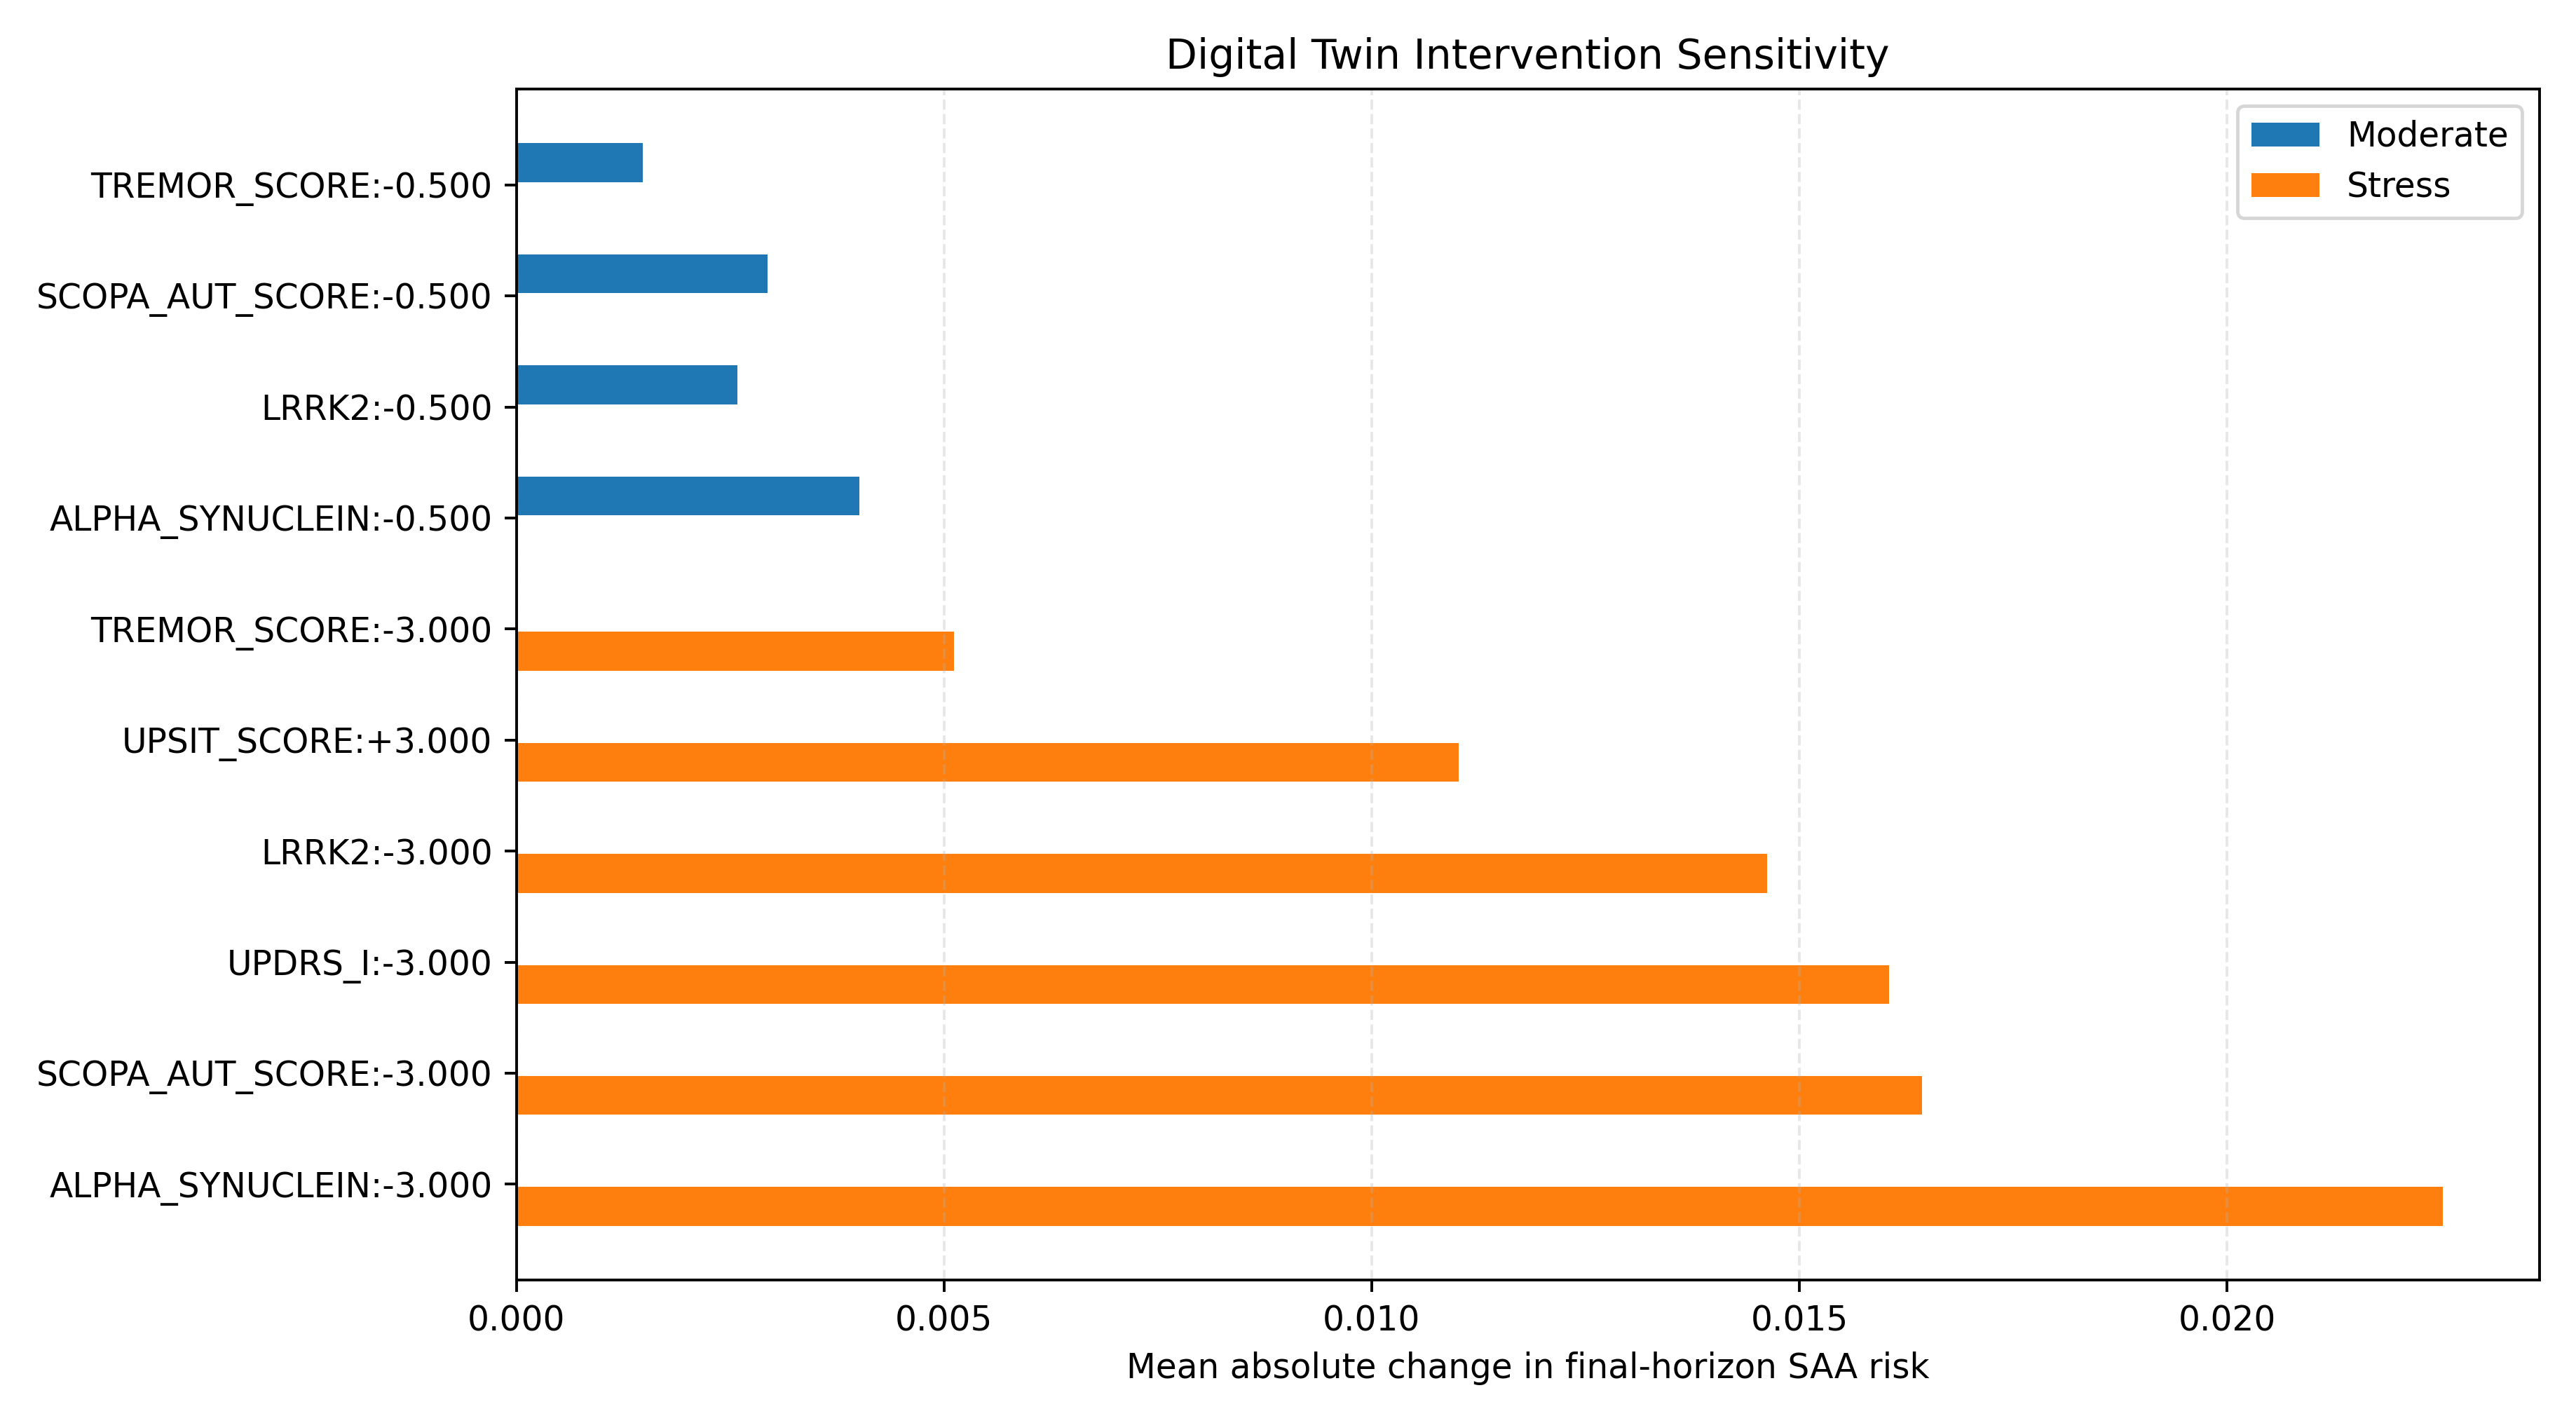
\includegraphics[width=0.95\textwidth]{../../../visualizations/publication_ieee/Figure04_DigitalTwin_Sensitivity.png}
\caption{Digital twin intervention sensitivity outputs.}
\label{fig:twin}
\end{figure*}

\section{Discussion}
The principal advance of this work is methodological hardening rather than headline performance escalation. The framework now couples model development with explicit governance: deterministic preprocessing, machine-readable validation artifacts, calibration-first interpretation, and claim gating. This structure is essential for clinical ML studies where optimism bias can emerge from selective metric reporting.

The main unresolved barrier is transportability. Internal discrimination and explainability are competitive, but external-like performance remains weak under disjoint pull conditions. The appropriate claim boundary is therefore ``internally validated and externally testable,'' not ``clinically deployed'' or ``state-of-the-art in practice.'' This distinction is consistent with reporting guidance for prediction models \cite{moons2012risk,collins2015tripod}.

\subsection{Clinical and translational implications}
Three translational implications follow from these findings. First, calibrated probabilities must be treated as a first-class output; raw logits are inadequate for clinical risk communication. Second, modality readiness is not equivalent to modality utility; raw DICOM/NIfTI availability requires deterministic harmonization before promotion into canonical contracts. Third, external protocol failures are informative and should drive study design (sample composition, endpoint prevalence, and covariate completeness) rather than post hoc metric reframing.

\subsection{Dissertation impact and roadmap}
For dissertation-scale progress, the roadmap is now concrete and auditable:
\begin{enumerate}
\item expand high-value modalities (medication exposure, adverse-event trajectories, richer temporal visit dynamics),
\item execute locked-protocol external validation on independent cohorts,
\item operationalize near-real-time digital twin refresh with drift monitoring, recalibration checks, and intervention-audit traces.
\end{enumerate}
This progression preserves scientific rigor while enabling a defensible path from model development to clinical decision-support research.

\section{Limitations}
\begin{itemize}
\item External evidence currently reflects an external-like disjoint pull, not a fully independent consortium cohort.
\item Severe class imbalance and sparse events limit precision and survival discrimination in external-like runs.
\item Some subgroup analyses are underpowered or unavailable because key covariates are absent in the disjoint pull.
\item Digital twin refresh evaluation is currently strongest for bounded sensitivity and determinism; prospective clinical utility testing remains pending.
\item Clinical deployment requires additional governance, monitoring, prospective validation, and human-factors integration.
\end{itemize}

\section{Conclusion}
FUZZY GIMAN now supports an IEEE-grade, artifact-backed workflow for PD prognosis research: deterministic contracts, explainable outputs, calibration diagnostics, hardening gates, and pull-based external evaluation. Internal evidence supports model maturity for rigorous research use, while external-like evidence clearly indicates that transportability remains the dominant gap.

Accordingly, the model should be framed as clinically validation-ready rather than deployment-ready. The highest-value next step is independent external validation under the same locked protocol, followed by iterative digital twin update studies that quantify real-world stability and intervention relevance.

\section*{Acknowledgment}
The authors acknowledge PPMI participants and data contributors. AI-assisted tooling was used for manuscript drafting support and reproducibility workflow acceleration.

\section*{References}
\begin{thebibliography}{00}

\bibitem{dorsey2018parkinsons}
E. R. Dorsey et al., ``The emerging evidence of the Parkinson pandemic,'' \textit{Journal of Parkinson's Disease}, vol. 8, no. s1, pp. S3--S8, 2018.

\bibitem{schapira2017nonmotor}
A. H. V. Schapira et al., ``Non-motor features of Parkinson disease,'' \textit{Nature Reviews Neuroscience}, vol. 18, no. 7, pp. 435--450, 2017.

\bibitem{fereshtehnejad2017clinical}
S.-M. Fereshtehnejad et al., ``Clinical criteria for subtyping Parkinson's disease: biomarkers and longitudinal progression,'' \textit{Brain}, vol. 140, no. 7, pp. 1959--1976, 2017.

\bibitem{poewe2017parkinson}
W. Poewe et al., ``Parkinson disease,'' \textit{Nature Reviews Disease Primers}, vol. 3, no. 1, p. 17013, 2017.

\bibitem{goetz2008movement}
C. G. Goetz et al., ``Movement Disorder Society-sponsored revision of the Unified Parkinson's Disease Rating Scale (MDS-UPDRS),'' \textit{Movement Disorders}, vol. 23, no. 15, pp. 2129--2170, 2008.

\bibitem{kuncheva2010fuzzy}
L. I. Kuncheva and F. Steimann, ``Fuzzy diagnosis,'' \textit{Artificial Intelligence in Medicine}, vol. 16, no. 2, pp. 121--128, 1999.

\bibitem{torres2006fuzzy}
A. Torres and J. J. Nieto, ``Fuzzy logic in medicine and bioinformatics,'' \textit{Journal of Biomedicine and Biotechnology}, vol. 2006, Article ID 91908, 2006.

\bibitem{zadeh1994soft}
L. A. Zadeh, ``Fuzzy logic, neural networks, and soft computing,'' \textit{Communications of the ACM}, vol. 37, no. 3, pp. 77--84, 1994.

\bibitem{zadeh1965fuzzy}
L. A. Zadeh, ``Fuzzy sets,'' \textit{Information and Control}, vol. 8, no. 3, pp. 338--353, 1965.

\bibitem{lecun2015deep}
Y. LeCun, Y. Bengio, and G. Hinton, ``Deep learning,'' \textit{Nature}, vol. 521, no. 7553, pp. 436--444, 2015.

\bibitem{goldberg1989genetic}
D. E. Goldberg, \textit{Genetic Algorithms in Search, Optimization, and Machine Learning}. Addison-Wesley, 1989.

\bibitem{marek2011ppmi}
K. Marek et al., ``The Parkinson Progression Marker Initiative (PPMI),'' \textit{Progress in Neurobiology}, vol. 95, no. 4, pp. 629--635, 2011.

\bibitem{hett2019multimodal}
K. Hett et al., ``Multimodal hippocampal subfield grading for Alzheimer's disease classification,'' \textit{Scientific Reports}, vol. 9, no. 1, p. 13845, 2019.

\bibitem{el2019predicting}
I. El-Gazzar et al., ``Predicting Parkinson's disease progression from clinical and imaging data,'' \textit{Neurobiology of Aging}, vol. 81, pp. 49--57, 2019.

\bibitem{holzinger2019causability}
A. Holzinger et al., ``Causability and explainability of artificial intelligence in medicine,'' \textit{Wiley Interdisciplinary Reviews: Data Mining and Knowledge Discovery}, vol. 9, no. 4, p. e1312, 2019.

\bibitem{wu2020comprehensive}
Z. Wu et al., ``A comprehensive survey on graph neural networks,'' \textit{IEEE Transactions on Neural Networks and Learning Systems}, vol. 32, no. 1, pp. 4--24, 2021.

\bibitem{zitnik2018modeling}
M. Zitnik et al., ``Modeling polypharmacy side effects with graph convolutional networks,'' \textit{Bioinformatics}, vol. 34, no. 13, pp. i457--i466, 2018.

\bibitem{duvenaud2015convolutional}
D. K. Duvenaud et al., ``Convolutional networks on graphs for learning molecular fingerprints,'' in \textit{Advances in Neural Information Processing Systems}, vol. 28, 2015.

\bibitem{parisot2018disease}
S. Parisot et al., ``Disease prediction using graph convolutional networks: Application to autism spectrum disorder and Alzheimer's disease,'' \textit{Medical Image Analysis}, vol. 48, pp. 117--130, 2018.

\bibitem{velickovic2018graph}
P. Velickovic et al., ``Graph attention networks,'' in \textit{Proc. Int. Conf. Learning Representations}, 2018.

\bibitem{shu2021disease}
L. Shu et al., ``Disease prediction with edge-variational graph convolutional networks,'' \textit{Medical Image Analysis}, vol. 70, p. 102036, 2021.

\bibitem{pota2013fuzzy}
M. Pota et al., ``A fuzzy logic approach for ambient assisted living,'' in \textit{Proc. IEEE Int. Conf. Fuzzy Systems}, 2013, pp. 1--6.

\bibitem{kadhim2011designed}
M. A. Kadhim et al., ``Designed Fuzzy Expert System for Chronic Diseases Diagnosis,'' \textit{Babil}, vol. 1,no. 2, pp. 167--176, 2011.

\bibitem{nauck1997neuro}
D. Nauck et al., \textit{Foundations of Neuro-Fuzzy Systems}. John Wiley \& Sons, 1997.

\bibitem{guzman2005medical}
J. A. Guzman and S. C. Mettler, ``Statistical and fuzzy inference approach to medical diagnosis,'' in \textit{Proc. Int. Fuzzy Systems Conf.}, 2005.

\bibitem{bezdek1981pattern}
J. C. Bezdek, \textit{Pattern Recognition with Fuzzy Objective Function Algorithms}. Springer Science \& Business Media, 1981.

\bibitem{jang1993anfis}
J.-S. R. Jang, ``ANFIS: Adaptive-network-based fuzzy inference system,'' \textit{IEEE Transactions on Systems, Man, and Cybernetics}, vol. 23, no. 3, pp. 665--685, 1993.

\bibitem{baltrusaitis2018multimodal}
T. Baltrusaitis et al., ``Multimodal machine learning: A survey and taxonomy,'' \textit{IEEE Transactions on Pattern Analysis and Machine Intelligence}, vol. 41, no. 2, pp. 423--443, 2019.

\bibitem{marek2001dopamine}
K. Marek et al., ``[$^{123}$I] $\beta$-CIT SPECT imaging assessment of the rate of Parkinson's disease progression,'' \textit{Neurology}, vol. 57, no. 11, pp. 2089--2094, 2001.

\bibitem{bai2018recurrent}
S. Bai et al., ``An empirical evaluation of generic convolutional and recurrent networks for sequence modeling,'' \textit{arXiv preprint arXiv:1803.01271}, 2018.

\bibitem{wen20203d}
J. Wen et al., ``Convolutional neural networks for classification of Alzheimer's disease: Overview and reproducible evaluation,'' \textit{Medical Image Analysis}, vol. 63, p. 101694, 2020.

\bibitem{choi2016doctor}
E. Choi et al., ``Doctor AI: Predicting clinical events via recurrent neural networks,'' in \textit{Machine Learning for Healthcare Conf.}, 2016, pp. 301--318.

\bibitem{nalls2019identification}
M. A. Nalls et al., ``Identification of novel risk loci, causal insights, and heritable risk for Parkinson's disease: a meta-analysis of genome-wide association studies,'' \textit{The Lancet Neurology}, vol. 18, no. 12, pp. 1091--1102, 2019.

\bibitem{ji2021dnabert}
Y. Ji et al., ``DNABERT: pre-trained bidirectional encoder representations from transformers model for DNA-language in genome,'' \textit{Bioinformatics}, vol. 37, no. 15, pp. 2112--2120, 2021.

\bibitem{avsec2021effective}
Z. Avsec et al., ``Effective gene expression prediction from sequence by integrating long-range interactions,'' \textit{Nature Methods}, vol. 18, no. 10, pp. 1196--1203, 2021.

\bibitem{holden2018progression}
S. K. Holden et al., ``Progression of MDS-UPDRS scores over five years in de novo Parkinson disease from the Parkinson's progression markers initiative cohort,'' \textit{Movement Disorders Clinical Practice}, vol. 5, no. 1, pp. 47--53, 2018.

\bibitem{che2018recurrent}
Z. Che et al., ``Recurrent neural networks for multivariate time series with missing values,'' \textit{Scientific Reports}, vol. 8, no. 1, p. 6085, 2018.

\bibitem{katzman2018deepsurv}
J. L. Katzman et al., ``DeepSurv: personalized treatment recommender system using a Cox proportional hazards deep neural network,'' \textit{BMC Medical Research Methodology}, vol. 18, no. 1, p. 24, 2018.

\bibitem{li2018deeper}
Q. Li et al., ``Deeper insights into graph convolutional networks for semi-supervised learning,'' in \textit{Proc. AAAI Conf. Artificial Intelligence}, 2018.

\bibitem{wang2015differentiable}
G. Wang et al., ``Differentiable soft quantization: Bridging full-precision and low-bit neural networks,'' \textit{arXiv preprint arXiv:1908.05033}, 2019.

\bibitem{ying2019gnnexplainer}
R. Ying et al., ``GNNExplainer: Generating explanations for graph neural networks,'' in \textit{Advances in Neural Information Processing Systems}, vol. 32, 2019.

\bibitem{guo2017calibration}
C. Guo et al., ``On calibration of modern neural networks,'' in \textit{Proc. Int. Conf. Machine Learning}, 2017, pp. 1321--1330.

\bibitem{moons2012risk}
K. G. M. Moons et al., ``Risk prediction models: I. Development, internal validation, and assessing the incremental value of a new (bio)marker,'' \textit{Heart}, vol. 98, no. 9, pp. 683--690, 2012.

\bibitem{hamilton2017inductive}
W. L. Hamilton et al., ``Inductive representation learning on large graphs,'' in \textit{Advances in Neural Information Processing Systems}, vol. 30, 2017.

\bibitem{rudin2019stop}
C. Rudin, ``Stop explaining black box machine learning models for high stakes decisions and use interpretable models instead,'' \textit{Nature Machine Intelligence}, vol. 1, no. 5, pp. 206--215, 2019.

\bibitem{peters2017elements}
J. Peters et al., \textit{Elements of Causal Inference: Foundations and Learning Algorithms}. MIT Press, 2017.

\bibitem{kairouz2019advances}
P. Kairouz et al., ``Advances and open problems in federated learning,'' \textit{arXiv preprint arXiv:1912.04977}, 2019.

\bibitem{kazemi2020representation}
S. M. Kazemi et al., ``Representation learning for dynamic graphs: A survey,'' \textit{Journal of Machine Learning Research}, vol. 21, pp. 1--73, 2020.

\bibitem{litjens2017survey}
G. Litjens et al., ``A survey on deep learning in medical image analysis,'' \textit{Medical Image Analysis}, vol. 42, pp. 60--88, 2017.

\bibitem{eraslan2019deep}
G. Eraslan et al., ``Deep learning: new computational modelling techniques for genomics,'' \textit{Nature Reviews Genetics}, vol. 20, no. 7, pp. 389--403, 2019.

\bibitem{rajkomar2019machine}
A. Rajkomar et al., ``Machine learning in medicine,'' \textit{New England Journal of Medicine}, vol. 380, no. 14, pp. 1347--1358, 2019.

\bibitem{adeli2010fuzzy}
A. Adeli and M. Neshat, ``A fuzzy expert system for heart disease diagnosis,'' in \textit{Proc. Int. Multi-Conf. Engineers Computer Scientists}, 2010.

\bibitem{vickers2006decision}
A. J. Vickers and E. B. Elkin, ``Decision curve analysis: a novel method for evaluating prediction models,'' \textit{Medical Decision Making}, vol. 26, no. 6, pp. 565--574, 2006.

\bibitem{lundberg2017unified}
S. M. Lundberg and S.-I. Lee, ``A unified approach to interpreting model predictions,'' in \textit{Advances in Neural Information Processing Systems}, vol. 30, 2017.

\bibitem{van2019calibration}
B. Van Calster et al., ``Calibration: the Achilles heel of predictive analytics,'' \textit{BMC Medicine}, vol. 17, no. 1, p. 230, 2019.

\bibitem{collins2015tripod}
G. S. Collins et al., ``Transparent reporting of a multivariable prediction model for individual prognosis or diagnosis (TRIPOD): the TRIPOD statement,'' \textit{BMJ}, vol. 350, p. g7594, 2015.

\end{thebibliography}

\end{document}
